%% main.tex — Dissertação de Mestrado
%% FFCLRP-USP — Programa de Pós-Graduação em Computação Aplicada
%% Autor: Cássio Silva Takarada
%% Orientador: Prof. Dr. Luiz Otávio Murta Junior

\documentclass[
  12pt,
  openright,
  twoside,
  a4paper,
  english,
  brazil,
]{abntex2}

%% ─── Pacotes ────────────────────────────────────────────────────────────────
\usepackage[T1]{fontenc}
\usepackage[utf8]{inputenc}
\usepackage{lmodern}
\usepackage{microtype}
\usepackage{amsmath,amssymb}
\usepackage{graphicx}
\usepackage{float}
\usepackage{booktabs}
\usepackage{multirow}
\usepackage{siunitx}
\usepackage{hyperref}
\usepackage{cleveref}
\usepackage[alf,abnt-emphasize=bf]{abntex2cite}  % ABNT author-year citations (wraps natbib)
\usepackage{claudedraft}     % orange draft environment for AI-generated passages

%% ─── Metadados ───────────────────────────────────────────────────────────────
\titulo{Complexidade Estatística dos Pesos de Redes Neurais Profundas como Marcador de Overfitting}
\autor{Cássio Silva Takarada}
\local{Ribeirão Preto}
\data{2025}
\orientador{Prof. Dr. Luiz Otávio Murta Junior}
\instituicao{Universidade de São Paulo \\ Faculdade de Filosofia, Ciências e Letras de Ribeirão Preto}
\tipotrabalho{Dissertação de Mestrado}

\preambulo{Dissertação apresentada ao Programa de Pós-Graduação em Computação
Aplicada da Faculdade de Filosofia, Ciências e Letras de Ribeirão Preto da
Universidade de São Paulo, como parte dos requisitos para obtenção do título
de Mestre em Ciências.}

%% ─── Hifenização ─────────────────────────────────────────────────────────────
\hyphenation{over-fitting under-fitting}

\begin{document}

\selectlanguage{brazil}
\frenchspacing

%% ─── Elementos pré-textuais ──────────────────────────────────────────────────
\imprimircapa
\imprimirfolhaderosto*
\tableofcontents
\listoffigures
\listoftables

%% ─── Corpo ───────────────────────────────────────────────────────────────────
\textual

%% capitulos/introducao.tex — Capítulo 1: Introdução
%%
%% Bloco escrito por Claude com base na qualificação de 2025 e em buscas
%% bibliográficas no scite (DOIs verificados). Conteúdo revisado e aprovado;
%% a marcação de rascunho foi removida em 2026-09-29.

\chapter{Introdução}
\label{ch:introducao}

% WRITER:BEGIN:introducao/full

\section{Contexto da análise de imagens médicas no diagnóstico clínico}
\label{sec:intro-contexto}

A imagem médica consolidou-se como um dos pilares do diagnóstico clínico
contemporâneo. Modalidades como tomografia computadorizada, ressonância
magnética, radiografia, ultrassonografia, tomografia por emissão de pósitrons
e a histopatologia digital fornecem representações detalhadas de estruturas
internas e teciduais que sustentam decisões de triagem, estadiamento e
acompanhamento terapêutico em praticamente todas as especialidades médicas
\cite{jiang2023}. O volume de dados gerado por esses exames cresce de modo
contínuo, ao mesmo tempo em que sua interpretação permanece uma tarefa que
exige treinamento especializado e está sujeita a variabilidade inter e
intraobservador. Esse cenário motiva o desenvolvimento de ferramentas
computacionais capazes de oferecer suporte quantitativo à análise dessas
imagens, notadamente em tarefas de classificação, segmentação e detecção
de anomalias.

\section{Avanços em aprendizado profundo aplicados à medicina}
\label{sec:intro-dl}

Nas últimas décadas o aprendizado profundo (\emph{deep learning}, DL)
emergiu como o paradigma dominante para o processamento de imagens médicas.
Em particular, redes neurais convolucionais profundas, exemplificadas pela
família de redes residuais introduzida por \citeonline{he2016}, alcançaram
desempenho próximo ou superior ao de especialistas humanos em diversas
tarefas de classificação e detecção \cite{jiang2023}. Esse progresso é
sustentado, de um lado, pelo aumento sistemático do poder computacional e,
de outro, pela disponibilização de coleções públicas padronizadas de imagens
médicas que viabilizam treinamento, comparação e reprodutibilidade de
modelos. Entre essas coleções destaca-se o \emph{benchmark} MedMNIST v2
\cite{medmnist2023}, que reúne dezoito conjuntos de classificação 2D e 3D
oriundos de patologia, radiologia e oftalmologia, padronizados em baixa
resolução para permitir prototipagem rápida sem perder representatividade
das modalidades clínicas.

Apesar desses avanços, modelos profundos operam de modo essencialmente
opaco do ponto de vista clínico: a relação entre os parâmetros aprendidos
e as decisões de saída não é trivialmente legível, configurando o problema
classicamente designado por \emph{caixa-preta}. Levantamentos recentes
apontam que essa limitação constitui hoje a principal barreira à adoção
de DL em fluxos diagnósticos sensíveis, mais relevante até que o ganho
marginal de acurácia em métricas tradicionais \cite{teng2022}. Nesse
contexto, a interpretabilidade dos modelos depende não apenas de explicações
\emph{post hoc} sobre saídas individuais, mas também de instrumentos
quantitativos que caracterizem o estado interno da rede durante o
treinamento.

\section{Justificativa do uso de medidas de complexidade}
\label{sec:intro-justificativa}

Métricas tradicionais de avaliação --- acurácia, perda de validação,
área sob a curva ROC --- capturam o comportamento do modelo sobre um
conjunto de dados específico, mas não oferecem leitura direta sobre a
organização estatística dos pesos aprendidos. Essa lacuna é particularmente
visível no fenômeno do \emph{overfitting}: redes com elevada capacidade
podem memorizar o conjunto de treinamento de modo a atingir acurácia
quase perfeita sobre ele, ao mesmo tempo em que generalizam mal para
dados novos. Análises teóricas recentes da dinâmica de generalização em
regimes de alta dimensionalidade indicam que os pesos atravessam fases
qualitativamente distintas durante o treinamento, com implicações diretas
sobre a capacidade preditiva do modelo \cite{advani2020}, e métodos
dedicados à detecção de \emph{overfitting} em aplicações clínicas têm
sido propostos como resposta prática a esse problema \cite{zhang2025}.

A presente dissertação parte da hipótese de que medidas de complexidade
aplicadas diretamente aos pesos da rede podem servir como marcadores
objetivos da maturação do treinamento e do início do sobreajuste. Duas
famílias de medidas dão sustentação a essa abordagem. A primeira é a
Entropia de Amostra (\emph{Sample Entropy}, SampEn) introduzida por
\citeonline{richman2000} como refinamento da Entropia Aproximada de
\citeonline{pincus1991}; SampEn quantifica, sem viés sistemático associado a
contagens de auto-coincidência, a regularidade de uma sequência de valores
e tem aplicação consolidada na análise de sinais fisiológicos. Sua extensão
bidimensional, SampEn2D, foi formalizada por \citeonline{silva2016} para
caracterizar a irregularidade de texturas espaciais em imagens biomédicas,
e é diretamente aplicável à matriz de pesos de uma camada convolucional.
A análise multiescala (Multiscale Entropy, MSE) proposta por
\citeonline{costa2002} complementa SampEn ao revelar regularidades que se
manifestam em diferentes resoluções da mesma sequência ou matriz.

A segunda família é a complexidade estatística de López-Ruiz, Mancini e
Calbet \cite{lmc1995}, definida pelo produto entre uma medida de
incerteza, tipicamente a entropia de Shannon, e uma medida de
desequilíbrio em relação à distribuição uniforme. Diferentemente de
medidas puramente entrópicas, a complexidade LMC anula-se nos extremos
de ordem perfeita e desordem perfeita, atingindo valores máximos em
regimes intermediários de auto-organização \cite{anteneodo1996}.
Aplicada à distribuição dos pesos de uma rede neural, espera-se que ela
descreva quantitativamente a transição entre o estado inicial aleatório
e o estado treinado. A combinação entre SampEn (sensível à estrutura
sequencial e espacial dos pesos) e LMC (sensível à forma da distribuição
marginal) constitui o eixo metodológico desta investigação.

\subsection{Justificativa prática: o ponto de vista de quem treina a rede}
\label{sec:intro-just-dev}

A justificativa apresentada até aqui é de natureza metodológica: as medidas de
complexidade oferecem uma leitura dos pesos que as métricas de desempenho não
oferecem. Há, porém, uma segunda justificativa, de natureza prática, que motiva
este trabalho de modo mais imediato e é formulada deliberadamente do ponto de
vista de quem desenvolve e treina a rede.

\subsubsection*{A dependência atual dos dados rotulados}

Para saber se uma rede aprendeu ou apenas memorizou, o desenvolvedor depende
hoje, integralmente, dos dados. É preciso construir conjuntos de treino,
validação e teste bem particionados, corretamente rotulados e representativos da
população de interesse. Cada um desses requisitos custa tempo e recursos, e em
imagens médicas frequentemente esbarra na indisponibilidade de especialistas
para a anotação. O diagnóstico do treinamento é, portanto, função do orçamento
de anotação disponível --- e não uma propriedade que se possa ler diretamente do
modelo.

O procedimento padrão para decidir quando interromper o ajuste, a parada
antecipada, monitora o erro em um conjunto de validação separado
\cite{prechelt1998}. O procedimento é sólido, mas transfere ao conjunto de
validação toda a responsabilidade pelo diagnóstico: se ele é pequeno,
desbalanceado ou pouco representativo, a estimativa do momento de parada
torna-se ruidosa, e o desenvolvedor não dispõe de sinal alternativo com que
confrontá-la. Em outras palavras, justamente no regime de poucos dados ---
aquele em que o sobreajuste é mais provável --- o instrumento de medida é o
menos confiável.

\subsubsection*{O que muda com um indicador calculado sobre os pesos}

As medidas investigadas nesta dissertação são calculadas exclusivamente a partir
dos pesos. Não consomem imagem, não consomem rótulo e não dependem de nenhuma
partição. Caso sejam capazes de sinalizar a transição para o regime de
memorização, o desenvolvedor passa a dispor de uma segunda leitura do
treinamento, obtida por caminho independente daquele do conjunto de validação.
As duas leituras podem então ser confrontadas: quando concordam, a decisão de
parada ganha confiança; quando discordam, há indício de que a validação não é
representativa.

Note-se que a proposta não é substituir a parada antecipada clássica, cuja
fundamentação é sólida, mas acrescentar-lhe uma fonte de evidência independente.

\subsubsection*{Casos de uso}

\begin{enumerate}
    \item \textbf{Decidir quando interromper o treinamento.} Um aviso emitido
    antes da degradação observável na validação amplia a janela de decisão, em
    lugar de constatar a perda depois de consumada.

    \item \textbf{Economizar recursos computacionais.} Detectar que a rede
    deixou de aprender evita épocas de treinamento que não trarão ganho, com
    impacto direto no custo de processamento.

    \item \textbf{Comparar arquiteturas sem ampliar a anotação.} Como a medida
    não consome dados rotulados, a comparação entre arquiteturas candidatas não
    exige a ampliação do conjunto de validação.

    \item \textbf{Diagnosticar quando a validação é pequena.} Em cenários nos
    quais o conjunto de validação é pequeno demais para ser confiável, um
    indicador independente fornece evidência adicional --- precisamente o cenário
    típico em imagens médicas.
\end{enumerate}

\subsubsection*{Entrega prática e delimitação}

A contribuição não se esgota na constatação empírica. Entrega-se um monitor
implementado em PyTorch, acoplável ao laço de treinamento de terceiros, que
calcula os indicadores a cada época e devolve um estado do aprendizado, conforme
descrito na Seção~\ref{sec:monitor}. O custo computacional é baixo quando a
medida incide sobre a camada densa.

Registre-se, por honestidade, que a utilidade prática aqui descrita é
\emph{condicional} ao sucesso empírico dos indicadores, e que os resultados do
Capítulo~\ref{ch:resultados} mostram que esse sucesso não é uniforme: depende da
medida empregada. As implicações dessa delimitação para o uso prático são
discutidas no Capítulo~\ref{ch:conclusao}.

\section{Hipótese, objetivos e escopo}
\label{sec:intro-objetivos}

A hipótese central deste trabalho é que a complexidade estatística dos
pesos de uma rede neural profunda evolui de modo sistemático durante
o treinamento e constitui um marcador objetivo do início do
\emph{overfitting}. Mais especificamente, postula-se que a trajetória
das medidas LMC e SampEn ao longo dos passos de otimização exibe
inflexão não monotônica, e que essa inflexão precede ou coincide com a
saturação da acurácia de validação.

A pesquisa adota um \textbf{escopo deliberadamente restrito} a fim de
permitir o controle das variáveis de interesse e a reprodutibilidade
plena dos experimentos:

\begin{itemize}
  \item \textbf{Arquitetura:} ResNet-18 \cite{he2016}, escolhida
        por sua importância histórica, profundidade moderada e papel de
        \emph{baseline} consagrado em classificação de imagens médicas;
        parte dos experimentos é repetida com a DenseNet-121 para
        verificar a dependência em relação à arquitetura.
  \item \textbf{Conjunto de dados:} MedNIST, com seis classes de imagens
        médicas de diferentes modalidades (Seção~\ref{sec:dados}).
  \item \textbf{Pesos analisados:} apenas os da camada densa
        (classificadora), calculando-se as medidas sobre a camada inteira.
  \item \textbf{Tarefa única:} classificação multiclasse, excluindo-se
        explicitamente segmentação semântica, detecção e tarefas
        ordinais.
\end{itemize}

Arquiteturas alternativas como U-Net, conjuntos de dados de maior escala
como NIH ChestX-ray14 e TCIA, e tarefas adicionais como segmentação ---
mencionados no projeto de qualificação --- ficam relegados a trabalhos
futuros (\autoref{ch:conclusao}).

Os objetivos específicos são:

\begin{enumerate}
  \item Implementar SampEn1D, SampEn2D e a complexidade LMC com
        validação numérica em casos analiticamente conhecidos
        (distribuições uniforme, gaussiana e séries periódicas), conforme
        o \autoref{ap:validacao-numerica}.
  \item Extrair os pesos da camada densa a cada época, durante o
        treinamento, excluindo o vetor de viés da análise.
  \item Calcular a trajetória das medidas de complexidade em execuções
        com corrupção de rótulos e em seus controles pareados, e
        confrontá-la com a evolução da perda e da acurácia de validação.
  \item Avaliar se a inflexão das trajetórias LMC e SampEn coincide,
        antecipa ou sucede o início observável do sobreajuste, e
        comparar os comportamentos entre níveis de corrupção e entre
        arquiteturas.
\end{enumerate}

\section{Organização do trabalho}
\label{sec:intro-organizacao}

O restante desta dissertação está organizado em quatro capítulos. O
\autoref{ch:fundamentacao} apresenta a fundamentação teórica das
medidas de complexidade utilizadas (Entropia de Shannon, ApEn, SampEn,
SampEn2D, complexidade LMC) e situa-as no contexto da literatura
de redes neurais profundas e análise de séries de pesos. O
\autoref{ch:metodologia} descreve o conjunto de dados, as arquiteturas,
o protocolo de treinamento, a indução de memorização por corrupção de
rótulos, a camada densa como objeto de medida e os parâmetros adotados
para cada medida ($m$, $r$, número de \emph{bins}). O
\autoref{ch:resultados} apresenta as trajetórias de complexidade da
camada densa nas execuções com corrupção de rótulos e em seus controles
pareados, e sua relação com a perda e a acurácia de validação. O
\autoref{ch:conclusao} sintetiza as evidências obtidas em relação à
hipótese central, discute as limitações do recorte adotado e indica
direções para extensões futuras envolvendo arquiteturas, modalidades
de imagem e tarefas adicionais.

% WRITER:END:introducao/full

%% capitulos/fundamentacao.tex — Capítulo 2: Fundamentação Teórica
%%
%% Bloco 1 (Conteúdo Teórico) escrito por Claude com base em buscas
%% bibliográficas no scite (DOIs verificados). Sinalizado em laranja itálico
%% pelo ambiente claudedraft. Trave a seção quando o conteúdo for aprovado:
%%   python -m src.writer --lock fundamentacao/conteudo

\chapter{Fundamentação Teórica}
\label{ch:fundamentacao}

% WRITER:BEGIN:fundamentacao/conteudo
\begin{claudedraft}

Este capítulo apresenta o aparato conceitual e operacional sobre o qual
se constrói a metodologia da dissertação. A
\autoref{sec:teoria-informacao} retoma a entropia de Shannon e seus
desdobramentos em entropia diferencial e divergências, dando base
formal às medidas que vêm a seguir. A \autoref{sec:apen-sampen}
percorre a transição da Entropia Aproximada (ApEn) para a Entropia de
Amostra (SampEn), explicitando os vieses que motivaram o refinamento e
a interpretação probabilística de SampEn como log-verossimilhança
condicional. As \autoref{sec:sampen2d} e \autoref{sec:mse} estendem
SampEn ao domínio espacial bidimensional e ao plano multiescala,
respectivamente, fornecendo as duas leituras complementares sobre a
matriz de pesos de uma camada convolucional. Por fim, a
\autoref{sec:lmc} apresenta a complexidade estatística de López-Ruiz,
Mancini e Calbet (LMC), discute a controvérsia sobre normalização e
intensividade que se seguiu à proposta original e justifica a
convenção $C = H \times D$ adotada no restante do trabalho.

\section{Sistemas complexos, auto-organização e emergência}
\label{sec:sistemas-complexos}

Esta seção fixa o vocabulário conceitual sobre o qual as medidas das seções
seguintes se apoiam. A justificativa para sua presença é direta: o restante
desta dissertação afirma que os pesos de uma rede em treinamento apresentam
regimes de \emph{auto-organização}, e essa afirmação não tem conteúdo
verificável enquanto o termo não for definido.

\subsection{A noção de sistema complexo}

Um sistema complexo pode ser informalmente caracterizado como uma rede de
muitos componentes que interagem entre si e cujo comportamento coletivo surge e
evolui por auto-organização \cite{sayama2015}. A caracterização carrega duas
exigências que não são triviais. A primeira é a \emph{multiplicidade} de
componentes interagentes. A segunda, mais restritiva, é que a informação
relevante do sistema resida nas \emph{relações} entre as partes, e não nas
partes isoladamente; se o comportamento do todo for recuperável pela simples
soma dos comportamentos individuais, o sistema é agregado, não complexo.

Uma rede neural profunda em treinamento satisfaz ambas as exigências. Os
milhões de pesos constituem componentes que interagem indiretamente, pela
retropropagação do gradiente, e nenhum peso isolado codifica a função aprendida
--- o conteúdo do modelo está na configuração conjunta. Essa observação não é
retórica: é ela que autoriza aplicar ao treinamento o instrumental
desenvolvido para sistemas complexos, em lugar de tratar a rede apenas como um
problema de otimização de alta dimensão.

\subsection{Emergência}

Denomina-se \emph{emergente} a propriedade que se manifesta no nível
macroscópico do sistema e que não é redutível às propriedades dos componentes
isolados \cite{sayama2015}. O conceito exige, portanto, a distinção explícita de
dois níveis de descrição: o microscópico, dos componentes, e o macroscópico, do
comportamento observável.

Na presente dissertação essa distinção é operacional, e não apenas conceitual.
O nível microscópico é o dos valores individuais dos pesos; o macroscópico é o
da capacidade de generalização do modelo, aferida em dados não vistos. A
hipótese central pode então ser reformulada nesses termos: pretende-se
verificar se uma estatística calculada sobre o nível microscópico --- a
distribuição e a organização dos pesos --- acompanha, e eventualmente antecipa,
a transição de regime observada no nível macroscópico.

\subsection{Auto-organização}

Chama-se \emph{auto-organização} ao processo pelo qual um sistema desenvolve
estrutura macroscópica sem que essa estrutura seja imposta por um controle
externo ou por um plano centralizado \cite{sayama2015}. Emergência e
auto-organização são conceitos distintos, ainda que frequentemente tratados como
sinônimos: a primeira descreve uma relação entre níveis de descrição em um
instante, e a segunda descreve a evolução temporal do sistema.

O treinamento por descida de gradiente é, nessa acepção, um processo de
auto-organização. Nenhum agente externo especifica o valor que cada peso deve
assumir; os valores resultam da aplicação iterada de uma regra local de
atualização, e a estrutura que se observa ao final --- filtros que respondem a
padrões visuais, camadas que se especializam --- não foi projetada peso a peso.

Interessa particularmente a este trabalho a observação de que sistemas em
auto-organização não evoluem de modo homogêneo: eles frequentemente apresentam
\emph{transições de regime}, nas quais o comportamento qualitativo muda em
intervalos relativamente curtos \cite{sayama2015}. É exatamente essa a estrutura
que a hipótese desta dissertação pressupõe. Se o treinamento consistisse em um
processo homogêneo de melhoria gradual, não haveria transição a ser detectada, e
a busca por um marcador do início do sobreajuste careceria de objeto. A
existência de dois regimes sucessivos no aprendizado --- um em que a rede extrai
regularidades generalizáveis e outro em que passa a memorizar exemplos
inconsistentes --- é documentada empiricamente por
\citeonline{arpit2017} e constitui o pressuposto factual da proposta.

\subsection{Delimitação: o que não se pretende afirmar}

Convém delimitar o alcance do enquadramento para evitar leitura excessiva. O
aparato de sistemas complexos é empregado aqui em sentido \emph{descritivo}, e
não como apelo a um mecanismo explicativo. Não se afirma que o treinamento de
uma rede neural seja formalmente equivalente a algum dos modelos canônicos da
área --- autômatos celulares, sistemas de reação-difusão ou redes dinâmicas
\cite{sayama2015} ---, nem se pretende derivar as medidas empregadas a partir de
primeiros princípios da teoria de sistemas complexos.

O que o enquadramento fornece é mais modesto e suficiente: a legitimidade de
tratar a configuração dos pesos como estado de um sistema cuja organização
macroscópica varia no tempo, e cujas transições podem, em princípio, ser
detectadas por estatísticas calculadas sobre esse estado. As medidas
específicas utilizadas provêm da teoria da informação e da análise de séries,
apresentadas nas seções seguintes, e sua validade é estabelecida empiricamente
no Capítulo~\ref{ch:resultados}, não por filiação teórica.

\section{Entropia de Shannon e teoria da informação}
\label{sec:teoria-informacao}

A entropia de Shannon \cite{shannon1948} é a pedra angular sobre a
qual se assenta toda a discussão subsequente. Para uma variável
aleatória discreta $X$ que assume valores no alfabeto finito
$\mathcal{X} = \{x_1, x_2, \ldots, x_N\}$ com distribuição de
probabilidade $P = (p_1, p_2, \ldots, p_N)$, a entropia é definida por
\begin{equation}
  H(X) = -\sum_{i=1}^{N} p_i \log_2 p_i,
  \label{eq:shannon-discrete}
\end{equation}
adotando-se, por convenção, $0 \log_2 0 = 0$. A escolha do logaritmo
na base $2$ implica que $H$ é medida em bits, interpretação
diretamente associada ao número médio mínimo de dígitos binários
necessário para codificar uma realização de $X$. A entropia satisfaz
$0 \le H(X) \le \log_2 N$, com extremos alcançados, respectivamente,
pela distribuição degenerada (existe $i$ tal que $p_i = 1$) e pela
distribuição uniforme ($p_i = 1/N$ para todo $i$). Caracterizações
axiomáticas mostram que essas propriedades, junto da continuidade e da
aditividade, determinam $H$ a menos de um fator multiplicativo
\cite{coverthomas2006}.

Quando $X$ é uma variável contínua com função de densidade de
probabilidade $f$, a generalização natural --- a entropia diferencial
--- é dada por
\begin{equation}
  h(X) = -\int_{\mathcal{X}} f(x) \log_2 f(x)\, dx,
  \label{eq:shannon-diff}
\end{equation}
sempre que a integral exista. Diferentemente da versão discreta,
$h(X)$ pode assumir valores negativos e não é invariante sob mudança
de escala, o que limita seu uso direto como índice de
``incerteza''. Em aplicações práticas com pesos de redes neurais,
trabalha-se com a versão discretizada por meio de histogramas com $N$
bins, recuperando a forma da \autoref{eq:shannon-discrete} a um custo
controlado de viés e variância \cite{coverthomas2006}.

Uma medida de dissimilaridade entre duas distribuições $P$ e $Q$
sobre o mesmo alfabeto é a divergência de Kullback--Leibler
\begin{equation}
  D_{\mathrm{KL}}(P\|Q) = \sum_{i=1}^{N} p_i \log_2 \frac{p_i}{q_i},
  \label{eq:kl}
\end{equation}
que é não negativa e nula se, e somente se, $P = Q$. A
\autoref{eq:kl} é central nesta dissertação porque a noção de
``desequilíbrio'' subjacente à complexidade LMC pode ser interpretada
como uma medida de afastamento entre $P$ e a distribuição de
referência (uniforme), tema retomado na \autoref{sec:lmc}.

\section{Entropia Aproximada e Entropia de Amostra}
\label{sec:apen-sampen}

O salto da teoria da informação para a análise de séries temporais
finitas exige um estimador de regularidade que opere com poucos pontos
e seja robusto a ruído moderado. A Entropia Aproximada (ApEn),
introduzida por \citeonline{pincus1991}, foi a primeira proposta a
preencher esse papel para sinais fisiológicos. Dada uma série
$\mathbf{u} = (u_1, u_2, \ldots, u_N)$, fixa-se um comprimento de
embedding $m$ e uma tolerância $r$ e constroem-se os vetores
$\mathbf{x}_i = (u_i, u_{i+1}, \ldots, u_{i+m-1})$ com
$1 \le i \le N - m + 1$. Para cada $i$ define-se
\begin{equation}
  C_i^m(r) = \frac{\#\{j : d[\mathbf{x}_i, \mathbf{x}_j] \le r\}}
                  {N - m + 1},
  \label{eq:apen-ci}
\end{equation}
onde $d[\cdot, \cdot]$ é a distância de Chebyshev (máximo das
diferenças absolutas componente a componente) e a contagem inclui o
caso $j = i$ (\emph{self-match}). A ApEn é então
\begin{equation}
  \mathrm{ApEn}(m, r, N) = \Phi^m(r) - \Phi^{m+1}(r),
  \quad
  \Phi^m(r) = \frac{1}{N - m + 1}\sum_{i=1}^{N-m+1} \ln C_i^m(r).
  \label{eq:apen}
\end{equation}

A inclusão de \emph{self-matches} em $C_i^m(r)$ é simultaneamente o
recurso que viabiliza a definição (evita logaritmo de zero) e a fonte
de seus dois principais defeitos: (i) ApEn é sistematicamente
enviesada para valores menores em séries curtas, e (ii) sua
consistência relativa --- a propriedade de que, ao se comparar duas
séries em um mesmo $r$, a ordem dos valores se preserva quando $r$
varia --- não é garantida \cite{richman2000,delgadobonal2019}. A
literatura subsequente documenta cenários em que classificações
fisiológicas baseadas em ApEn se invertem ao se mudar a tolerância,
comprometendo seu uso como marcador objetivo
\cite{yentes2013,delgadobonal2019}.

A Entropia de Amostra (SampEn), proposta por \citeonline{richman2000},
remove essas limitações por construção. Em vez de calcular o
logaritmo médio de probabilidades locais, conta-se globalmente o
número de pares de templates próximos. Sejam
\begin{align}
  B^m(r) &= \#\{(i, j) : i < j,\ d[\mathbf{x}_i, \mathbf{x}_j] \le r\},
  \label{eq:sampen-B} \\
  A^m(r) &= \#\{(i, j) : i < j,\ d[\mathbf{x}_i, \mathbf{x}_j] \le r,
                       \ |u_{i+m} - u_{j+m}| \le r\},
  \label{eq:sampen-A}
\end{align}
isto é, $B^m(r)$ conta pares de janelas de comprimento $m$ próximas e
$A^m(r)$ conta os pares dessas janelas que permanecem próximas após
um passo adicional. A SampEn é dada por
\begin{equation}
  \mathrm{SampEn}(m, r, N) = -\ln \frac{A^m(r)}{B^m(r)}.
  \label{eq:sampen}
\end{equation}
Pela construção, ambas as contagens excluem o par $(i, i)$, eliminando
o viés associado às auto-coincidências. A interpretação de
\autoref{eq:sampen} é direta e instrutiva: SampEn é o negativo do
logaritmo da probabilidade condicional de que duas janelas próximas
em comprimento $m$ permaneçam próximas em comprimento $m + 1$.
Valores baixos correspondem a séries muito regulares (a continuação
é altamente previsível); valores altos, a séries irregulares
(continuação imprevisível).

A \autoref{eq:sampen} herda independência tanto de $N$ quanto da
ordem dos pares por ser uma estatística baseada em razão de contagens
globais. Demonstrou-se ainda que, em uma ampla família de processos
estocásticos, SampEn possui consistência relativa entre tolerâncias,
propriedade que ApEn não satisfaz \cite{richman2000}. Por outro lado,
a literatura recente registra cenários particulares de processos do
tipo $\mathrm{MIX}$ contaminados por ruído em que mesmo SampEn pode
falhar essa consistência, recomendando cautela ao se interpretar
diferenças finas entre séries de naturezas distintas
\cite{delgadobonal2019}.

A escolha dos parâmetros $m$ e $r$ é prática consagrada na
literatura. Pela análise sistemática de \citeonline{yentes2013} sobre
séries curtas, recomenda-se $m = 2$ e $r$ entre $0{,}1$ e $0{,}25$ do
desvio padrão da série, com $N \ge 200$ para evitar instabilidade
estatística. Esta dissertação adota $m = 2$ e $r = 0{,}2 \times
\sigma$, com $\sigma$ tomado como desvio padrão populacional
(\texttt{ddof}=0), em consonância com a convenção do grupo de pesquisa
e com o intervalo recomendado pela literatura. Ressalva-se que tensores
pequenos --- em particular os parâmetros $\gamma$ e $\beta$ do
\emph{batch normalization} das camadas iniciais --- podem ter
comprimento inferior a $N = 200$, regime em que a estimativa de SampEn
é menos estável; esse limite é levado em conta na interpretação desses
grupos.

\section{Entropia de Amostra Bidimensional (SampEn2D)}
\label{sec:sampen2d}

A extensão bidimensional da SampEn surge da observação de que pesos
de camadas convolucionais e parâmetros de matrizes têm estrutura
espacial: a vizinhança de um peso é tão informativa quanto sua
sequência linear, e o domínio natural para análise é a matriz, não
o vetor. \citeonline{silva2014embc} apresentaram uma primeira
formulação, validada posteriormente em \citeonline{silva2016} sobre
imagens de textura sintéticas, do banco Brodatz e de cortes
histológicos de nervo sural, demonstrando que SampEn2D recupera as
propriedades qualitativas de SampEn 1D ao mesmo tempo em que
incorpora a dependência bidimensional.

Seja $\mathbf{W} \in \mathbb{R}^{H \times W}$ uma matriz de pesos
extraída de uma camada da rede. Fixe-se um tamanho de janela $m$ e
uma tolerância $r$. As janelas $m \times m$ centradas em
$(i, j)$ formam a coleção
$\mathcal{V}_m = \{ \mathbf{V}_{i,j}^{(m)} : 1 \le i \le H - m,\,
1 \le j \le W - m\}$. Para uma janela maior $(m+1) \times (m+1)$,
analogamente, escreve-se $\mathcal{V}_{m+1}$. Por construção,
restringe-se às posições $(i, j)$ tais que ambas as janelas $m$ e
$m+1$ caibam integralmente em $\mathbf{W}$, garantindo emparelhamento
entre $\mathcal{V}_m$ e $\mathcal{V}_{m+1}$. Em analogia com as
\autoref{eq:sampen-B} e \autoref{eq:sampen-A}, definem-se
\begin{align}
  B^m_{\mathrm{2D}}(r)
    &= \#\{(p, q) : p \neq q,\ d[\mathbf{V}_p^{(m)}, \mathbf{V}_q^{(m)}] \le r\},
    \label{eq:sampen2d-B} \\
  A^m_{\mathrm{2D}}(r)
    &= \#\{(p, q) : p \neq q,\ d[\mathbf{V}_p^{(m+1)}, \mathbf{V}_q^{(m+1)}] \le r\},
    \label{eq:sampen2d-A}
\end{align}
em que $p, q$ percorrem as posições válidas e $d[\cdot, \cdot]$ é a
distância de Chebyshev sobre a janela vista como vetor. A
\emph{Sample Entropy 2D} é
\begin{equation}
  \mathrm{SampEn2D}(m, r, \mathbf{W})
    = -\ln \frac{A^m_{\mathrm{2D}}(r)}{B^m_{\mathrm{2D}}(r)}.
  \label{eq:sampen2d}
\end{equation}
A interpretação probabilística replica a do caso unidimensional:
SampEn2D é o negativo do logaritmo da probabilidade de que duas
janelas $m \times m$ próximas tenham vizinhanças que permaneçam
próximas quando a janela é estendida em uma linha e uma coluna.

A literatura aponta dois aspectos práticos relevantes. Primeiro, a
SampEn2D pode produzir valores indefinidos para matrizes pequenas
quando $A^m_{\mathrm{2D}}(r) = 0$, problema que motivou propostas
alternativas baseadas em entropias de dispersão e
fuzzificação. Segundo, o custo computacional cresce
quadraticamente com o número de janelas válidas, tornando a
estimativa custosa para matrizes grandes \cite{silva2016}. Para os
fins desta dissertação, o tamanho típico das matrizes de uma camada
convolucional na ResNet-18 mantém-se confortavelmente acima do
regime patológico identificado pela literatura, e a SampEn2D é
aplicada diretamente, sem recurso a substitutos.

\section{Entropia Multiescala (MSE)}
\label{sec:mse}

A SampEn captura irregularidade em uma escala fixa. No entanto,
sistemas com correlações de longo alcance --- batimentos cardíacos
saudáveis, ruído $1/f$, dinâmica de redes complexas ---  apresentam
estrutura em múltiplas escalas temporais simultaneamente. A Entropia
Multiescala (MSE), proposta por \citeonline{costa2002} e
sistematizada em \citeonline{costa2005}, lê esse fenômeno por meio de
uma sequência de granulações grosseiras (\emph{coarse-grainings}) da
série original.

Dada uma série $\mathbf{u}$ e um fator de escala $\tau \in
\mathbb{N}^{\ast}$, constrói-se a série granulosa
\begin{equation}
  y_j^{(\tau)} = \frac{1}{\tau} \sum_{i = (j-1)\tau + 1}^{j\tau} u_i,
  \quad 1 \le j \le \lfloor N/\tau \rfloor,
  \label{eq:mse-coarse}
\end{equation}
isto é, médias de blocos não sobrepostos de comprimento $\tau$. A
escala $\tau = 1$ recupera a série original. Para cada $\tau$,
calcula-se SampEn da série granulosa, formando o perfil multiescala
$\{\mathrm{SampEn}(m, r, y^{(\tau)}) : \tau = 1, 2, \ldots,
\tau_{\max}\}$.

Um detalhe metodológico crítico: a tolerância $r$ é fixada uma única
vez a partir do desvio padrão da série \emph{original} e mantida
constante em todas as escalas, conforme prescrição de
\citeonline{costa2005}. Recomputar $r$ em cada escala invalidaria a
comparação entre escalas, pois mudanças no perfil de complexidade
ficariam confundidas com a renormalização local. A interpretação
qualitativa da curva $\mathrm{SampEn}$ versus $\tau$ separa três
classes principais: ruído branco (entropia decresce monotonicamente),
ruído $1/f$ (entropia constante ao longo das escalas) e periódicos
(entropia próxima de zero em todas as escalas). Sistemas
fisiológicos saudáveis apresentam padrão similar ao $1/f$,
enquanto patologias frequentemente colapsam para perfis
monotonicamente decrescentes \cite{costa2005}.

Esta dissertação aplica MSE 1D ao vetor de pesos achatado e, na
extensão proposta por \citeonline{silva2016} para SampEn2D, MSE 2D às
matrizes via granulação por blocos $\tau \times \tau$. Em ambos os
casos, $r$ é mantido fixo em $0{,}2 \times \sigma$ da matriz original,
com $\sigma$ calculado em população.

\section{Complexidade Estatística LMC}
\label{sec:lmc}

A entropia, isoladamente, não é uma boa medida de complexidade.
Distribuições uniformes (entropia máxima) são tão simples quanto
distribuições degeneradas (entropia mínima), no sentido de que ambas
são facilmente descritíveis e desprovidas de estrutura interna.
\citeonline{lmc1995}\,---\,doravante LMC\,---\,propuseram, como
remédio, uma medida que se anula em ambos os extremos e atinge
valores máximos em regimes intermediários de auto-organização. Para
uma distribuição $P = (p_1, \ldots, p_N)$, define-se o
\emph{desequilíbrio}
\begin{equation}
  D(P) = \sum_{i=1}^{N} \left( p_i - \frac{1}{N} \right)^{2},
  \label{eq:lmc-disequilibrium}
\end{equation}
isto é, o quadrado da distância $L_2$ até a distribuição uniforme.
A complexidade estatística LMC é o produto
\begin{equation}
  C(P) = H(P) \times D(P),
  \label{eq:lmc}
\end{equation}
em que $H$ é a entropia de Shannon, dada pela
\autoref{eq:shannon-discrete}. Como $H$ é máxima e $D$ é nula sob a
distribuição uniforme, e $H$ é nula e $D$ é máxima sob a distribuição
degenerada, $C$ se anula em ambos os extremos por construção. Para
distribuições intermediárias, $C$ assume valores estritamente
positivos, refletindo simultaneamente incerteza e afastamento do
equilíbrio \cite{lmc1995}.

A definição original gerou debate intenso. \citeonline{anteneodo1996}
demonstraram, no contexto de ensembles físicos, que $C$ na forma
\autoref{eq:lmc} \emph{não} é uma quantidade intensiva: ao se
duplicar o tamanho do sistema, $C$ não satisfaz a relação de
escala esperada de uma medida termodinâmica genuína. Esse fato
limita a transferibilidade direta de $C$ entre sistemas de
tamanhos distintos e motivou a busca por refinamentos.
\citeonline{feldman1998}, em uma revisão crítica das medidas de
complexidade estatística disponíveis na época, articularam três
desideratos: a medida deve (i) anular-se nos extremos de ordem e
desordem perfeitas, (ii) ser intensiva, e (iii) capturar a presença
de estrutura correlacional em escalas relevantes do sistema.

A resposta mais influente a essas críticas é a complexidade
estatística generalizada (SCM, \emph{Statistical Complexity
Measure}), introduzida por \citeonline{lamberti2004} e desenvolvida
por \citeonline{rosso2010}. Em vez do produto $H \times D$, define-se
\begin{equation}
  C_{\mathrm{SCM}}(P) = Q_J(P, P_e) \cdot H(P) / H_{\max},
  \label{eq:scm}
\end{equation}
em que $H_{\max} = \log_2 N$ normaliza a entropia, $P_e$ é a
distribuição de equilíbrio (tipicamente uniforme), e $Q_J(P, P_e)$ é
o desequilíbrio em divergência de Jensen-Shannon, normalizado de modo
que $0 \le Q_J \le 1$. A construção \autoref{eq:scm} é intensiva,
limitada ao intervalo $[0, 1]$ e aplicável a uma variedade de
sistemas dinâmicos contínuos e discretos.

Apesar das vantagens formais da SCM, esta dissertação adota a forma
original \autoref{eq:lmc}\,---\,$C = H \times D$ em bits, sem
normalização\,---\,por três razões metodológicas que merecem
explicitação:

\begin{enumerate}
  \item \textbf{Comparação intra-modelo, não inter-sistema.} O objeto
        de análise são as trajetórias de complexidade dos pesos de
        \emph{uma mesma rede} em \emph{um mesmo grupo de camadas} ao
        longo do treinamento. As comparações são pareadas por
        \emph{checkpoint}, \emph{seed} e dataset; o argumento de
        intensividade de \citeonline{anteneodo1996}, que diz respeito
        à escalonamento entre sistemas de tamanhos distintos, não é
        ativado nesse desenho experimental.
  \item \textbf{Sensibilidade a transições intermediárias.} A forma
        $H \times D$ é sensível justamente ao regime que interessa à
        hipótese central\,---\,a transição entre o estado inicial
        aleatório e o estado treinado. Versões normalizadas saturam
        nas extremidades do intervalo $[0, 1]$, comprimindo as
        diferenças que se busca medir. A versão não normalizada
        preserva a granularidade necessária para detectar inflexões
        sutis na trajetória.
  \item \textbf{Convenção do grupo de pesquisa.} Trabalhos anteriores
        do mesmo grupo \cite{silva2016,silva2012qsampen} adotam a
        convenção $H \times D$ em bits, sem normalização, com
        binarização adaptativa da forma $N = \min(100, \max(10,
        n/5))$, onde $n$ é o número de amostras. Manter essa
        convenção preserva a comparabilidade direta entre os
        resultados desta dissertação e os da literatura imediata.
\end{enumerate}

A normalização adaptativa do número de bins $N$ é especialmente
relevante para a aplicação a pesos de redes neurais, onde o número
de parâmetros varia ordens de grandeza entre camadas: tipicamente
poucas centenas em camadas iniciais e dezenas de milhares em
camadas profundas. A regra $N = \min(100, \max(10, n/5))$ garante
resolução suficiente para camadas pequenas sem incorrer em viés de
subamostragem em camadas grandes.

A combinação entre LMC (sensível à forma da distribuição marginal
dos pesos) e SampEn (sensível à estrutura sequencial e espacial)
fornece, portanto, dois ângulos complementares sobre o estado
interno da rede ao longo do treinamento. Os parâmetros operacionais
adotados, junto da fundamentação aqui apresentada, são retomados em
detalhe no \autoref{ch:metodologia}.

\end{claudedraft}

% ===========================================================================
\section{Estado da arte: leitura do estado interno de redes profundas}
\label{sec:trabalhos-relacionados}

Esta seção discute os trabalhos que se aproximam do problema desta dissertação.
O critério de seleção adotado foi a existência de alguma tentativa de
caracterizar o estado de generalização de uma rede a partir de seu
\emph{interior} --- pesos, representações ou dinâmica de treinamento --- em
lugar de aferi-lo exclusivamente pelo desempenho em dados rotulados. A
Seção~\ref{sec:ea-memorizacao} revisa o que se sabe sobre memorização. A
Seção~\ref{sec:ea-normas} discute a família de limites baseados em normas e
margens. A Seção~\ref{sec:ea-espectral} trata das abordagens espectrais. A
Seção~\ref{sec:ea-info} apresenta a família informação-teórica e a controvérsia
que a acompanha. A Seção~\ref{sec:ea-sintese} sintetiza e posiciona a proposta.

\subsection{Memorização e os dois regimes do aprendizado}
\label{sec:ea-memorizacao}

\citeonline{zhang2017} demonstraram que redes convolucionais de grande porte
ajustam perfeitamente rótulos atribuídos ao acaso, e que esse comportamento
persiste sob regularização explícita. O resultado é duplamente relevante para
esta dissertação: estabelece que a capacidade de memorização não é acidente, mas
propriedade das arquiteturas usuais, e fornece o protocolo de indução por
corrupção controlada de rótulos adotado no Capítulo~\ref{ch:metodologia}. A
limitação, do ponto de vista aqui assumido, é que o diagnóstico permanece
ancorado na comparação entre desempenho de treino e de teste.

\citeonline{arpit2017} refinam o quadro ao mostrar que memorização e aprendizado
de padrões não são simultâneos: redes tendem a aprender primeiro as
regularidades simples e só depois memorizar os exemplos ruidosos. A existência
de dois regimes sucessivos, e não de um processo homogêneo, é o pressuposto que
torna plausível a hipótese desta dissertação --- se há transição, pode haver
assinatura da transição. Os autores, contudo, caracterizam os regimes por
métricas que dependem dos dados, não da estrutura dos pesos.

\citeonline{power2022} descrevem o fenômeno de \emph{grokking}, em que a
generalização emerge muito depois do ajuste completo do treino, às vezes após
longo período de estagnação da validação. O fenômeno constitui contraexemplo aos
critérios ingênuos de parada antecipada: uma interrupção baseada apenas na
estagnação eliminaria justamente o regime em que a generalização acabaria por
surgir. Um indicador que leia o estado interno, e não apenas o desempenho
externo, é potencialmente capaz de distinguir estagnação de reorganização ---
questão registrada aqui como hipótese derivada, não testada neste trabalho.

\subsection{Limites de generalização por normas e margens}
\label{sec:ea-normas}

\citeonline{bartlett2017} propõem limites de generalização baseados em normas
espectrais e margens, estabelecendo que propriedades geométricas dos pesos se
relacionam com a capacidade de generalizar. \citeonline{dziugaite2017} obtêm,
por via PAC-Bayesiana, limites não vacuosos para redes sobreparametrizadas ---
resultado notável, dado que limites clássicos tornam-se vazios nesse regime.
Ambos representam avanços substantivos, mas produzem limites válidos para
\emph{um} estado da rede, tipicamente o final do treinamento, e não uma leitura
acompanhável ao longo das épocas.

\citeonline{jiang2020} conduzem o estudo empírico mais sistemático dessa
família, avaliando um grande conjunto de medidas candidatas quanto à sua relação
causal com a lacuna de generalização. A conclusão é cautelar e impõe exigência
metodológica a qualquer trabalho subsequente: muitas medidas teoricamente
motivadas correlacionam-se mal com a generalização observada, e medidas baseadas
em otimização desempenham-se melhor do que as baseadas em norma. A consequência
adotada nesta dissertação é que não basta exibir correlação entre indicador e
sobreajuste em uma execução; é preciso demonstrar \emph{discriminação} entre
execuções com e sem memorização, com controles pareados e teste de
significância.

\subsection{Abordagens espectrais}
\label{sec:ea-espectral}

\citeonline{martin2021} mostram que propriedades de cauda pesada do espectro das
matrizes de pesos permitem prever tendências de qualidade de modelos sem acesso
aos dados de treino ou de teste. Este é o trabalho mais próximo do objetivo aqui
perseguido, e convém explicitar as diferenças. A abordagem é \emph{espectral},
apoiando-se nos autovalores das matrizes, ao passo que a desta dissertação é
\emph{informação-teórica}, apoiando-se na distribuição de valores e na
organização espacial dos pesos. Além disso, o alvo em \citeonline{martin2021} é
comparar modelos já treinados, enquanto aqui o alvo é acompanhar a trajetória
temporal de um único treinamento.

\subsection{Abordagens informação-teóricas e a controvérsia do gargalo de informação}
\label{sec:ea-info}

A família mais próxima em espírito a esta dissertação é a que aplica teoria da
informação ao interior de redes profundas. \citeonline{tishby2015} propõem
analisar redes no \emph{plano de informação}, quantificando cada camada pela
informação mútua que preserva a respeito da entrada e da saída, e interpretam o
treinamento como otimização de um compromisso entre compressão e predição.
\citeonline{shwartzziv2017} desenvolvem empiricamente essa leitura e relatam
que a maior parte das épocas de treinamento é consumida não no ajuste dos
rótulos, mas na \emph{compressão} da representação, identificando duas fases
distintas na otimização --- uma de deriva rápida e outra de relaxação
estocástica.

A pertinência para o presente trabalho é evidente: trata-se de literatura que
afirma existirem transições de regime detectáveis por quantidades
informação-teóricas calculadas sobre o interior da rede, o que é precisamente a
estrutura da hipótese aqui investigada.

É imprescindível, porém, registrar que essas conclusões foram contestadas.
\citeonline{saxe2019} examinam os três principais postulados da teoria e
concluem que nenhum deles se sustenta no caso geral: a existência de duas fases
distintas, a relação causal entre compressão e boa generalização, e a atribuição
da compressão ao comportamento difusivo do gradiente estocástico. Demonstram, em
particular, que a trajetória observada no plano de informação depende
predominantemente da não linearidade empregada --- funções de saturação bilateral
produzem fase de compressão, enquanto ativações lineares ou de saturação
unilateral não a produzem --- e que parte do efeito reflete decisões de estimação
da informação mútua em redes determinísticas.

Essa controvérsia recomenda cautela e delimita o escopo do presente trabalho de
modo produtivo. As medidas aqui empregadas \emph{não} são estimativas de
informação mútua entre camadas e dados, e portanto não herdam as dificuldades de
estimação que Saxe e colaboradores identificam: LMC, SampEn e SampEn2D são
estatísticas calculadas sobre os \emph{valores dos pesos}, sem referência a
qualquer distribuição conjunta com os dados. A escolha evita o problema
metodológico central da controvérsia, ao custo de abdicar da interpretação
formal em termos de compressão de informação.

\subsection{Síntese e posicionamento da proposta}
\label{sec:ea-sintese}

\begin{table}[H]
\centering
\caption{Comparação dos trabalhos discutidos quanto à dependência de dados
rotulados, à natureza temporal da leitura e ao objeto medido.}
\label{tab:estado-arte}
\footnotesize
\begin{tabular}{llccc}
\toprule
\textbf{Trabalho} & \textbf{Objeto da medida} & \textbf{Exige rótulo} &
\textbf{Leitura temporal} & \textbf{Avisa antes} \\
\midrule
\citeonline{prechelt1998}   & Erro de validação          & Sim & Sim & Não \\
\citeonline{zhang2017}      & Desempenho                 & Sim & Não & Não \\
\citeonline{arpit2017}      & Desempenho                 & Sim & Sim & Não \\
\citeonline{bartlett2017}   & Norma espectral            & Não & Não & Não \\
\citeonline{dziugaite2017}  & Limite PAC-Bayes           & Sim & Não & Não \\
\citeonline{jiang2020}      & Diversas                   & Sim & Não & Não \\
\citeonline{martin2021}     & Espectro dos pesos         & Não & Não & Não \\
\citeonline{tishby2015}     & Informação mútua           & Sim & Não & Não \\
\citeonline{shwartzziv2017} & Informação mútua           & Sim & Sim & Não \\
\textbf{Esta dissertação}   & Complexidade dos pesos     & Não & Sim & Sim \\
\bottomrule
\end{tabular}
\fonte{Elaborado pelo autor.}
\end{table}

A Tabela~\ref{tab:estado-arte} organiza os trabalhos segundo três eixos. Quanto
à dependência de rótulos, apenas \citeonline{bartlett2017} e
\citeonline{martin2021} dispensam-nos, e ambos por via espectral. Quanto à
natureza temporal, \citeonline{arpit2017} e \citeonline{shwartzziv2017}
acompanham a trajetória do treinamento, mas ambos requerem acesso aos dados ---
o primeiro ao desempenho, o segundo à distribuição conjunta necessária para
estimar informação mútua. A intersecção entre \emph{dispensar rótulos} e
\emph{acompanhar a trajetória} permanece, até onde a revisão alcançou, não
ocupada.

A proposta desta dissertação situa-se nessa intersecção e diferencia-se da
literatura em quatro aspectos: (i) a medida é informação-teórica, mas incide
sobre a distribuição de valores e a organização espacial dos pesos, não sobre o
espectro das matrizes nem sobre informação mútua com os dados; (ii) a leitura é
temporal, produzindo uma trajetória por época em lugar de um escalar ao final do
treino; (iii) nenhum rótulo é consumido, o que a torna aplicável em cenários de
anotação escassa; e (iv) a validação é feita por controles estritamente pareados
com indução explícita de memorização, em resposta direta à advertência de
\citeonline{jiang2020} quanto a correlações espúrias.

Registre-se, por fim, uma limitação da própria revisão. A literatura de medidas
de generalização é extensa e cresce rapidamente; a seleção aqui apresentada
privilegiou trabalhos fundacionais de alta citação e os mais diretamente
relacionados ao problema, não constituindo revisão sistemática no sentido
metodológico do termo.

%% capitulos/metodologia.tex
%% Capítulo 3 — Metodologia

\chapter{Metodologia}
\label{ch:metodologia}

Este capítulo descreve o protocolo experimental adotado para investigar a
evolução da complexidade estatística dos pesos da camada densa de redes
neurais profundas durante o treinamento. A exposição segue do dado bruto às
medidas: o conjunto de dados (Seção~\ref{sec:dados}), as arquiteturas
(Seção~\ref{sec:arquitetura}) e o protocolo de treinamento
(Seção~\ref{sec:treinamento}); os regimes de treinamento comparados
(Seção~\ref{sec:regimes}); a camada densa como objeto de medida e a
ordem de achatamento dos seus pesos (Seção~\ref{sec:camada-densa}); as
medidas de complexidade (Seção~\ref{sec:medidas}); e o monitoramento durante o
treinamento (Seção~\ref{sec:monitor}).

% ===========================================================================
\section{Conjunto de dados}
\label{sec:dados}

Utiliza-se o MedNIST, conjunto de imagens médicas em escala de cinza,
$64 \times 64$ pixels, distribuídas em seis classes: tomografia abdominal
(\emph{AbdomenCT}), ressonância de mama (\emph{BreastMRI}), tomografia de
tórax (\emph{ChestCT}), radiografia de tórax (\emph{CXR}), radiografia de mão
(\emph{Hand}) e tomografia de crânio (\emph{HeadCT}). Emprega-se a partição
oficial do conjunto em treinamento, validação e teste, com
\num{47164}, \num{5895} e \num{5895} imagens, respectivamente. A semente que
define a partição é fixa em todas as execuções e distinta da semente de
inicialização dos pesos, de modo que todas as execuções compartilham
exatamente os mesmos conjuntos de validação e de teste. O conjunto de teste é
avaliado uma única vez por execução, ao final do treinamento.

% ===========================================================================
\section{Arquiteturas}
\label{sec:arquitetura}

Adota-se a ResNet-18 \cite{he2016} (implementação \texttt{torchvision},
sem pré-treinamento), com a camada totalmente conectada final substituída
para as seis classes do MedNIST. Esta arquitetura totaliza
aproximadamente $11{,}2$ milhões de parâmetros distribuídos em
\textbf{41 tensores com parâmetros aprendíveis}: 20 camadas convolucionais
(\texttt{Conv2d}), 20 camadas de \emph{batch normalization}
(\texttt{BatchNorm2d}) e 1 camada totalmente conectada (\texttt{Linear}),
que é o objeto das medidas deste trabalho
(Figura~\ref{fig:resnet-overview}).

\begin{figure}[H]
  \centering
  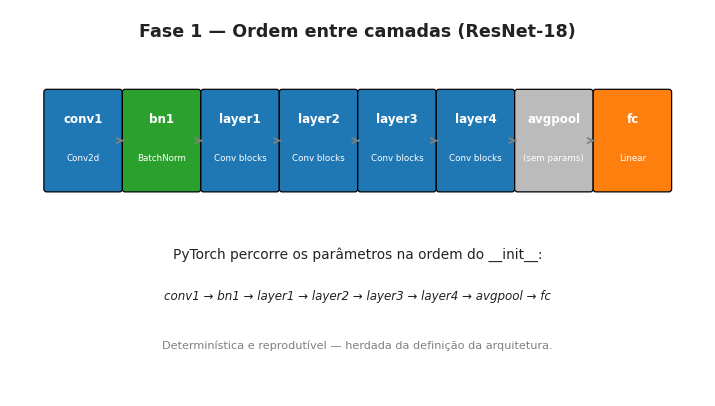
\includegraphics[width=0.95\linewidth]{figures/fig_resnet18_overview.png}
  \caption{Estrutura de nível superior da ResNet-18: oito módulos
  nomeados em sequência. As caixas indicam o tipo de camada
  (azul: Conv2d; verde: BatchNorm2d; cinza: sem parâmetros; laranja: Linear).
  As caixas \texttt{layer1}--\texttt{layer4} são contêineres
  \texttt{Sequential} de blocos residuais.}
  \label{fig:resnet-overview}
\end{figure}

Para descrever o comportamento das medidas em uma segunda arquitetura,
repetem-se as execuções de controle com a DenseNet-121 (implementação
\texttt{torchvision}, sem pré-treinamento), com a camada classificadora
igualmente substituída para seis classes.

% ===========================================================================
\section{Protocolo de treinamento}
\label{sec:treinamento}

O treinamento emprega o otimizador AdamW com taxa de aprendizado $10^{-3}$ e
\emph{weight decay} nulo, entropia cruzada como função objetivo, lotes de 128
imagens e 60 épocas, sem aumento de dados, salvo quando o regime exige outro
número de épocas (Seção~\ref{sec:subamostragem}). O \emph{weight decay} e o
aumento de dados são desligados deliberadamente: ambos são formas de
regularização, e mantê-los atribuiria a diferença entre regimes a mais de uma
causa. Todas as execuções compartilham essa configuração, de modo que cada
regime difere do controle apenas pelo fator manipulado.
Os experimentos foram executados em GPU (\emph{torch} $2{,}4{,}1$ e
\emph{torchvision} $0{,}19{,}1$).

% ===========================================================================
\section{Regimes de treinamento}
\label{sec:regimes}

As trajetórias das medidas são comparadas entre três regimes, todos com a
configuração da Seção~\ref{sec:treinamento}. Em cada regime, a semente que
governa a inicialização dos pesos varia entre as execuções, enquanto a partição
permanece fixa. Validação e teste nunca são alterados: o fator manipulado
incide \emph{apenas} sobre o treino, de modo que a validação mede o efeito
desse fator sobre a generalização.

\subsection{Controle}
\label{sec:controle}

O controle usa o conjunto de treino completo (\num{47164} imagens), com rótulos e
imagens intactos, por 60 épocas, o que corresponde a \num{22140} passos de
otimização (369 lotes por época). Na ResNet-18 há oito execuções de controle;
na DenseNet-121, cinco.

\subsection{Subamostragem do conjunto de treino}
\label{sec:subamostragem}

Treina-se com uma fração $f \in \{\SI{10}{\percent};\ \SI{2}{\percent};\
\SI{1}{\percent}\}$ do conjunto de treino, isto é, \num{4717}, \num{944} e
\num{471} imagens, com cinco sementes por fração. Reduzir o treino diminui
simultaneamente a quantidade de informação e a diversidade dos exemplos, e
torna o sobreajuste mais provável.

A subamostragem traz, porém, uma armadilha que precisa ser controlada.
Experimentos preliminares mostraram que, com poucos passos de otimização, as
estatísticas móveis das camadas de normalização em lote não convergem, e o
modelo colapsa em modo de avaliação --- inclusive sobre o próprio conjunto de
treino. O quadro se parece com sobreajuste catastrófico, mas o mesmo modelo
acerta cerca de \SI{94,5}{\percent} da validação quando a normalização usa as
estatísticas do lote corrente. Mede-se, nesse caso, um artefato de
normalização, e não perda de generalização.

Por isso cada fração é treinada em duas versões. Na versão \emph{curta}, o
número de épocas é o usual para a fração (60 épocas a \SI{10}{\percent} e 200
épocas a \SI{2}{\percent} e \SI{1}{\percent}, ou \num{2220}, \num{1600} e
\num{800} passos). Na versão de \emph{passos igualados}, o número de épocas é
ampliado até que o total de passos iguale o do controle (599, \num{2768} e
\num{5535} épocas, cerca de \num{22140} passos). A comparação entre as duas
versões separa o efeito de ter poucos dados do efeito de ter poucos passos.

\subsection{Ruído nas imagens de treino}
\label{sec:ruido-imagem}

Soma-se às imagens de treino um campo de ruído gerado no domínio da
frequência. Sorteia-se ruído branco gaussiano do tamanho da imagem, aplica-se a
transformada de Fourier bidimensional, multiplica-se o espectro pelo filtro
radial $1/f^{\beta/2}$, com $f$ a frequência espacial, e retorna-se ao domínio
espacial. O espectro de potência resultante é proporcional a $1/f^{\beta}$:
$\beta = 0$ produz ruído \emph{branco}, de potência plana, e $\beta = 1$
produz ruído \emph{rosa}, com mais potência nas baixas frequências. O
componente de frequência nula é zerado, para que o ruído não desloque o brilho
médio da imagem, e o campo é normalizado para desvio-padrão unitário. A imagem
ruidosa é $\mathrm{clip}(x + \sigma z,\ 0,\ 1)$, com $x$ a imagem em $[0, 1]$, $z$
o campo de ruído e $\sigma \in \{0{,}05;\ 0{,}1;\ 0{,}2\}$ a intensidade, na
mesma escala do pixel. O mesmo campo é somado aos três canais, pois o MedNIST é
escala de cinza replicada.

O ruído é \emph{fixo por imagem}: cada imagem de treino recebe sempre o mesmo
campo, em todas as épocas, de modo que a rede pode ajustá-lo. Os rótulos
permanecem intactos. Há cinco sementes por combinação de cor e intensidade,
totalizando 30 execuções.

% ===========================================================================

\section{A camada densa como objeto de medida}
\label{sec:camada-densa}

Seja a camada densa com $M$ entradas $x_1, \dots, x_M$ e $N$ neurônios
$n_1, \dots, n_N$. A matriz de pesos é $W \in \mathbb{R}^{N \times M}$, e
o elemento $w_{ji}$ é o peso do \emph{caminho} $x_i \rightarrow n_j$ ---
convenção que coincide com a forma nativa de \texttt{Linear.weight} no
PyTorch, $[\textrm{out\_features}, \textrm{in\_features}]$.

Como a SampEn$_{1D}$ compara janelas consecutivas, a ordem de achatamento
precisa ser fixada. Duas ordens são naturais. Na ordem \emph{por
neurônio}, percorrem-se todos os pesos que chegam a cada neurônio antes
de passar ao seguinte:

\begin{equation}
    v_{n} = (w_{11}, w_{12}, \dots, w_{1M},\; w_{21}, \dots, w_{2M},\; \dots,\; w_{NM}),
    \label{eq:ordem-neuronio}
\end{equation}

\noindent
o que corresponde ao achatamento nativo, sem transposição. Na ordem
\emph{por entrada}, percorrem-se todos os pesos que partem de cada
entrada:

\begin{equation}
    v_{x} = (w_{11}, w_{21}, \dots, w_{N1},\; w_{12}, \dots, w_{N2},\; \dots),
    \label{eq:ordem-entrada}
\end{equation}

\noindent
equivalente a transpor $W$ antes do achatamento. A
Equação~\ref{eq:ordem-neuronio} mede a regularidade \emph{dentro do campo
receptivo de cada neurônio}; a Equação~\ref{eq:ordem-entrada} mede a
regularidade \emph{da distribuição de uma mesma entrada entre os
neurônios}. Adota-se a primeira como convenção padrão, por corresponder ao
achatamento nativo do PyTorch. O Apêndice~\ref{ap:exemplo-numerico} ilustra as duas ordens
com um exemplo numérico. Para a complexidade LMC a distinção é
irrelevante, pois a medida depende apenas do histograma dos valores e é
invariante a permutações.

O vetor de viés é excluído da análise: o viés é um deslocamento aditivo
do neurônio, não a ligação entre uma entrada e um neurônio, e portanto
não é um caminho no sentido aqui adotado.

Na ResNet-18 aplicada a seis classes, a camada densa (\texttt{fc}) possui
$6 \times 512 = 3.072$ pesos; na DenseNet-121 (\texttt{classifier}),
$6 \times 1.024 = 6.144$. São quantidades que permitem calcular as medidas
sobre a camada inteira, sem subamostragem.

% ===========================================================================
\section{Medidas de complexidade}
\label{sec:medidas}

Sobre a camada densa de cada época são calculadas as medidas descritas a
seguir. Os parâmetros seguem convenções da literatura citada.

\subsection{Complexidade LMC}
\label{sec:medidas-lmc}

A complexidade estatística LMC \cite{lmc1995} é definida como o produto
da entropia de Shannon \cite{shannon1948} pelo desequilíbrio em relação
à distribuição uniforme:
\begin{equation}
  C_{\mathrm{LMC}}(p) \;=\; H(p) \cdot D(p),
\end{equation}
onde, para um histograma normalizado $p$ com $N$ \emph{bins},
\begin{equation}
  H(p) = -\sum_{i=1}^{N} p_i \log_2 p_i, \qquad
  D(p) = \sum_{i=1}^{N} \left(p_i - \tfrac{1}{N}\right)^2.
\end{equation}
Adota-se $N = 100$ \emph{bins}. A entropia é computada em bits ($\log_2$)
e o produto $H \cdot D$ é reportado sem normalização adicional. Como a
medida não é normalizada, sua escala depende de $N$, e nenhuma comparação
entre execuções é legítima sem que o número de intervalos seja idêntico.


\subsection{Entropia amostral SampEn$_{1D}$}
\label{sec:medidas-sampen}

A entropia amostral \cite{richman2000,pincus1991} é definida como
\begin{equation}
  \mathrm{SampEn}(U, m, r) \;=\;
  -\log \frac{A^{m+1}(r)}{B^{m}(r)},
\end{equation}
onde $U$ é o vetor de pesos achatado, $m$ é o comprimento das
sub-sequências comparadas e $r$ é a tolerância de similaridade. As
quantidades $A^{m+1}$ e $B^{m}$ contam pares de sub-sequências cuja
distância de Chebyshev é menor ou igual a $r$. Adotam-se os parâmetros
$m = 2$ e $r = 0{,}2\,\sigma(U)$ \cite{yentes2013}, validados pelo
grupo de pesquisa em estudos prévios.


% ===========================================================================

\section{Monitoramento durante o treinamento}
\label{sec:monitor}

As medidas são calculadas \textbf{a cada época, dentro do laço de
treinamento}, e não sobre \emph{snapshots} analisados posteriormente. A escolha
tem razão prática: nas execuções de passos igualados, com milhares de épocas,
guardar os pesos de cada época seria inviável em disco, e o cálculo dentro do
laço dispensa esse armazenamento.

São calculadas por época a complexidade LMC com $N_{bins} = 100$ e a
SampEn$_{1D}$ com $m = 2$ e $r = 0{,}20\,\sigma$.

O custo do monitoramento é baixo, pois incide apenas sobre a camada densa, e pode
ser desativado por opção de linha de comando.

%% capitulos/resultados.tex — Capítulo de Resultados

\chapter{Resultados}
\label{ch:resultados}

Este capítulo apresenta os resultados obtidos sobre a camada densa das redes
treinadas no MedNIST, segundo o protocolo descrito no
Capítulo~\ref{ch:metodologia}. Verifica-se, inicialmente, que a corrupção de
rótulos produziu memorização efetiva; em seguida, comparam-se as trajetórias da
LMC e das variantes de entropia amostral entre execuções com corrupção e seus
controles pareados, examinando o efeito do nível de corrupção, da arquitetura e
da ordem de achatamento dos pesos.

\section{Memorização induzida na camada densa}
\label{sec:res-desenho2}

Esta seção reporta os resultados do desenho descrito na
Seção~\ref{sec:desenho2}, no qual a perda de generalização é induzida por
corrupção de rótulos e as medidas incidem integralmente sobre os
\num{3072} pesos da camada densa. Todos os valores foram obtidos com
execuções de controle \emph{estritamente pareadas}, conforme discutido
adiante na Seção~\ref{sec:res-d2-pareamento}.

\subsection{Confirmação da memorização}
\label{sec:res-d2-memorizacao}

Antes de avaliar os indicadores, é necessário verificar que o protocolo
produziu de fato memorização, e não apenas degradação de desempenho. A
Tabela~\ref{tab:d2-memorizacao} apresenta a evidência nas oito execuções com
$\rho = 0{,}30$, isto é, \SI{25}{\percent} de rótulos efetivamente errados.

\begin{table}[H]
\centering
\caption{Evidência de memorização nas oito execuções com corrupção de rótulos
e nos oito controles pareados, em ResNet-18. Acurácias em modo de avaliação.}
\label{tab:d2-memorizacao}
\small
\begin{tabular}{lcccc}
\toprule
\textbf{Grupo} & \textbf{Treino inicial} & \textbf{Treino final} &
\textbf{Validação máxima} & \textbf{Validação final} \\
\midrule
Com corrupção ($n=8$) & \SI{74,7}{\percent} & \SI{97,5}{\percent} &
\SI{99,9}{\percent} & \SI{84,1}{\percent} \\
Controle pareado ($n=8$) & --- & \SI{100,0}{\percent} & \SI{100,0}{\percent} &
\SI{100,0}{\percent} \\
\bottomrule
\end{tabular}
\fonte{Elaborado pelo autor.}
\end{table}

O padrão é inequívoco e reprodutível nas oito execuções. A acurácia de treino
parte de aproximadamente \SI{74,7}{\percent} --- valor próximo do teto
imposto pelos rótulos corrompidos --- e sobe até \SI{97,5}{\percent}, o que
significa que a rede ajustou também a maior parte das associações
inconsistentes. Simultaneamente, a acurácia de validação, que chega a
\SI{99,9}{\percent}, regride para \SI{84,1}{\percent}. Não há explicação
visual para rótulos sorteados ao acaso; o único modo de ajustá-los é
memorizá-los. Nos controles pareados, treino e validação permanecem em
\SI{100}{\percent}, sem qualquer degradação --- o que confirma que a
memorização observada decorre da corrupção, e não do protocolo de
treinamento.

\begin{figure}[H]
    \centering
    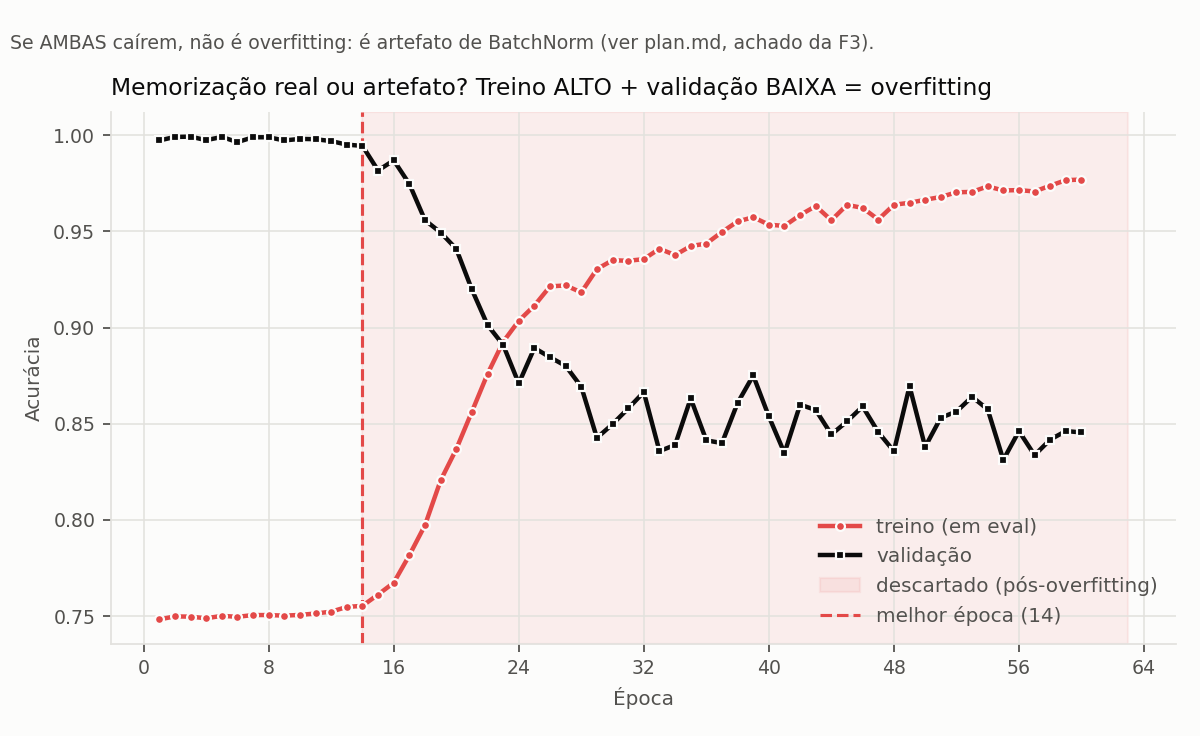
\includegraphics[width=0.9\textwidth]{figures/d2_memorizacao_resnet.png}
    \caption{Acurácias de treino, em modo de avaliação, e de validação ao longo
    das épocas em execução com \SI{25}{\percent} de rótulos efetivamente
    errados. O cruzamento das curvas caracteriza a memorização.}
    \label{fig:d2-memorizacao}
    \fonte{Elaborado pelo autor.}
\end{figure}

\subsection{Poder de discriminação dos indicadores}
\label{sec:res-d2-discriminacao}

O critério de avaliação adotado não é a amplitude absoluta de variação de cada
indicador, mas a \emph{razão} entre a amplitude observada nas execuções com
corrupção e a observada nos controles. Um indicador que varia muito nas duas
condições não informa nada sobre a memorização. A
Tabela~\ref{tab:d2-discriminacao} apresenta os resultados.

\begin{table}[H]
\centering
\caption{Amplitude de variação dos indicadores na camada densa, em ResNet-18,
com oito execuções por grupo. Valores como média $\pm$ desvio-padrão amostral;
$p$ obtido por teste de Mann-Whitney bilateral.}
\label{tab:d2-discriminacao}
\small
\begin{tabular}{lcccc}
\toprule
\textbf{Indicador} & \textbf{Com corrupção} & \textbf{Controle pareado} &
\textbf{Razão} & \textbf{$p$} \\
\midrule
LMC       & $1{,}219 \pm 0{,}055$ & $1{,}138 \pm 0{,}134$ & $1{,}07$ & $0{,}195$ \\
SampEn 1D & $0{,}205 \pm 0{,}018$ & $0{,}058 \pm 0{,}012$ & $3{,}51$ & $0{,}00016$ \\
SampEn2D  & $0{,}340 \pm 0{,}061$ & $0{,}060 \pm 0{,}014$ & $5{,}65$ & $0{,}00016$ \\
\bottomrule
\end{tabular}
\fonte{Elaborado pelo autor.}
\end{table}

O resultado é assimétrico e exige leitura cuidadosa. As duas variantes de
entropia amostral discriminam as condições, e a bidimensional discrimina
melhor. O valor $p = \num{0,00016}$ é o menor alcançável pelo teste de
Mann-Whitney com oito observações por grupo e corresponde à separação completa
entre os grupos, sem qualquer sobreposição de valores.

A complexidade LMC, em contrapartida, \textbf{não discrimina} as duas
condições. A razão de $1{,}07$ é compatível com ausência de efeito, e o teste
não rejeita a hipótese nula ($p = \num{0,195}$). Este é um resultado negativo,
e não uma limitação de potência: a amplitude média da LMC nas execuções com
corrupção ($1{,}219$) situa-se dentro de um desvio-padrão da amplitude média
dos controles ($1{,}138 \pm 0{,}134$).

A interpretação mais econômica desse achado remete à propriedade discutida na
Seção~\ref{sec:lmc}: a LMC depende apenas do histograma dos valores
dos pesos e é, portanto, invariante a qualquer permutação. Se a memorização
reorganiza os pesos da camada densa sem alterar substancialmente a
\emph{distribuição} de seus valores, a LMC é cega a ela por construção. As
variantes de entropia amostral, sensíveis à ordem, captam precisamente essa
reorganização.

\begin{figure}[H]
    \centering
    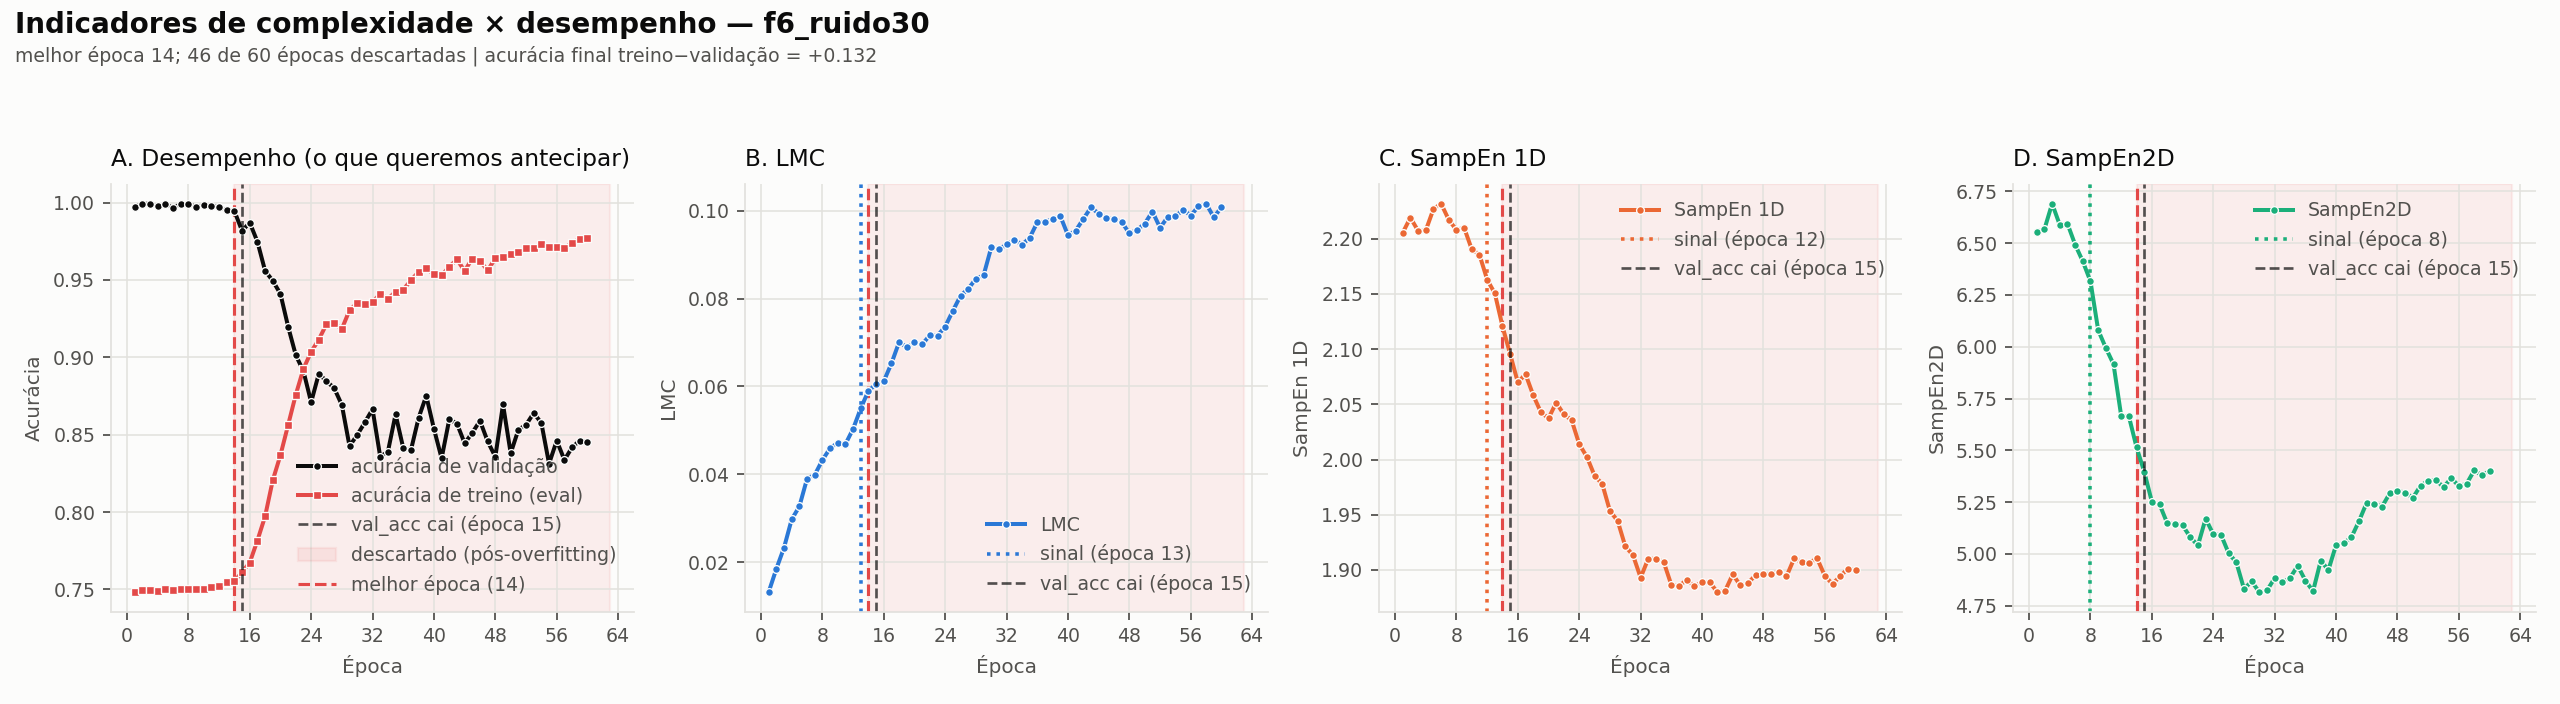
\includegraphics[width=0.95\textwidth]{figures/d2_indicadores_resnet.png}
    \caption{Trajetória dos três indicadores na camada densa e das curvas de
    validação, em execução com corrupção de rótulos. A região sombreada
    corresponde às épocas posteriores ao início do sobreajuste, excluídas das
    conclusões.}
    \label{fig:d2-indicadores}
    \fonte{Elaborado pelo autor.}
\end{figure}

\subsection{Antecedência em relação à degradação da validação}
\label{sec:res-d2-antecedencia}

A antecedência é a diferença, em épocas, entre a inflexão do indicador e a
âncora definida sobre a acurácia de validação. A
Tabela~\ref{tab:d2-antecedencia} reporta os valores.

\begin{table}[H]
\centering
\caption{Antecedência dos indicadores em relação à queda sustentada da acurácia
de validação, em épocas, nas oito execuções com corrupção em ResNet-18.}
\label{tab:d2-antecedencia}
\small
\begin{tabular}{lccc}
\toprule
\textbf{Indicador} & \textbf{Média $\pm$ desvio} & \textbf{IC \SI{95}{\percent}} &
\textbf{Discrimina?} \\
\midrule
SampEn2D  & $7{,}50 \pm 0{,}93$ & $[6{,}73;\ 8{,}27]$ & Sim \\
SampEn 1D & $3{,}62 \pm 1{,}06$ & $[2{,}74;\ 4{,}51]$ & Sim \\
LMC       & $3{,}00 \pm 1{,}85$ & $[1{,}45;\ 4{,}55]$ & Não \\
\bottomrule
\end{tabular}
\fonte{Elaborado pelo autor.}
\end{table}

A antecedência da LMC não constitui resultado positivo e não deve ser
interpretada como tal. Como a Tabela~\ref{tab:d2-discriminacao} estabelece que
o indicador não distingue as duas condições, a época de sua inflexão não
sinaliza coisa alguma: uma inflexão que ocorre igualmente nos controles não é
aviso. A antecedência só é informativa para indicadores que previamente
demonstraram discriminação.

A separação temporal da SampEn2D é quase completa. Nas oito execuções com
corrupção, o indicador inflete nas épocas $\{7,7,7,7,7,7,8,9\}$. Nos controles
pareados, seis dos oito inflectem, e o fazem nas épocas
$\{9,23,37,42,50,55\}$; os dois restantes não inflectem dentro do horizonte de
\num{60} épocas. Registre-se a honestidade do limite: há \emph{um} controle que
inflete na época \num{9}, coincidindo com o valor máximo observado no grupo com
corrupção. A separação é portanto quase perfeita, mas não perfeita, e a
afirmação correta é de sobreposição mínima --- em uma de dezesseis execuções.

\subsection{Efeito do nível de corrupção}
\label{sec:res-d2-niveis}

Variou-se a fração sorteada em $\rho \in \{0{,}15;\ 0{,}30;\ 0{,}50\}$, com três
sementes por nível. O resultado não era o esperado e é, talvez, o mais
interessante desta seção.

\begin{table}[H]
\centering
\caption{Época do alerta emitido pelo monitor e época da âncora, por nível de
corrupção, com três sementes por nível.}
\label{tab:d2-niveis}
\small
\begin{tabular}{lcccc}
\toprule
\textbf{$\rho$ sorteado} & \textbf{Errados de fato} & \textbf{Época do alerta} &
\textbf{Época da âncora} & \textbf{Antecedência} \\
\midrule
\SI{15}{\percent} & \SI{12,5}{\percent} & $10{,}0$ & $17{,}7$ & $7{,}7$ \\
\SI{30}{\percent} & \SI{25,0}{\percent} & $9{,}3$  & $14{,}7$ & $5{,}3$ \\
\SI{50}{\percent} & \SI{41,7}{\percent} & $10{,}0$ & $13{,}0$ & $3{,}0$ \\
\midrule
\multicolumn{2}{l}{ANOVA de uma via} & $F = 1{,}00$ & $F = 30{,}2$ & \\
\multicolumn{2}{l}{} & $p = 0{,}42$ & $p = 0{,}0007$ & \\
\bottomrule
\end{tabular}
\fonte{Elaborado pelo autor.}
\end{table}

A época em que o monitor emite o alerta é praticamente invariante ao nível de
corrupção: médias de $10{,}0$, $9{,}3$ e $10{,}0$ épocas, sem diferença
estatisticamente detectável ($F = \num{1,00}$; $p = \num{0,42}$). O que se move
é a âncora, isto é, o momento em que a degradação se torna visível na
validação, que chega progressivamente mais cedo quanto maior a corrupção
($F = \num{30,2}$; $p = \num{0,0007}$).

A consequência prática é que a antecedência encolhe à medida que a corrupção
aumenta, de aproximadamente $7{,}7$ épocas a \SI{15}{\percent} para $3{,}0$
épocas a \SI{50}{\percent}. Propõe-se a seguinte leitura: o indicador marca o
\emph{início} da memorização, cujo momento depende pouco da quantidade de
rótulos errados, enquanto a validação mede o \emph{sintoma}, que se manifesta
tanto mais cedo quanto maior a corrupção. Trata-se de interpretação
plausível e compatível com os dados, ainda não demonstrada de forma
independente.

\begin{figure}[H]
    \centering
    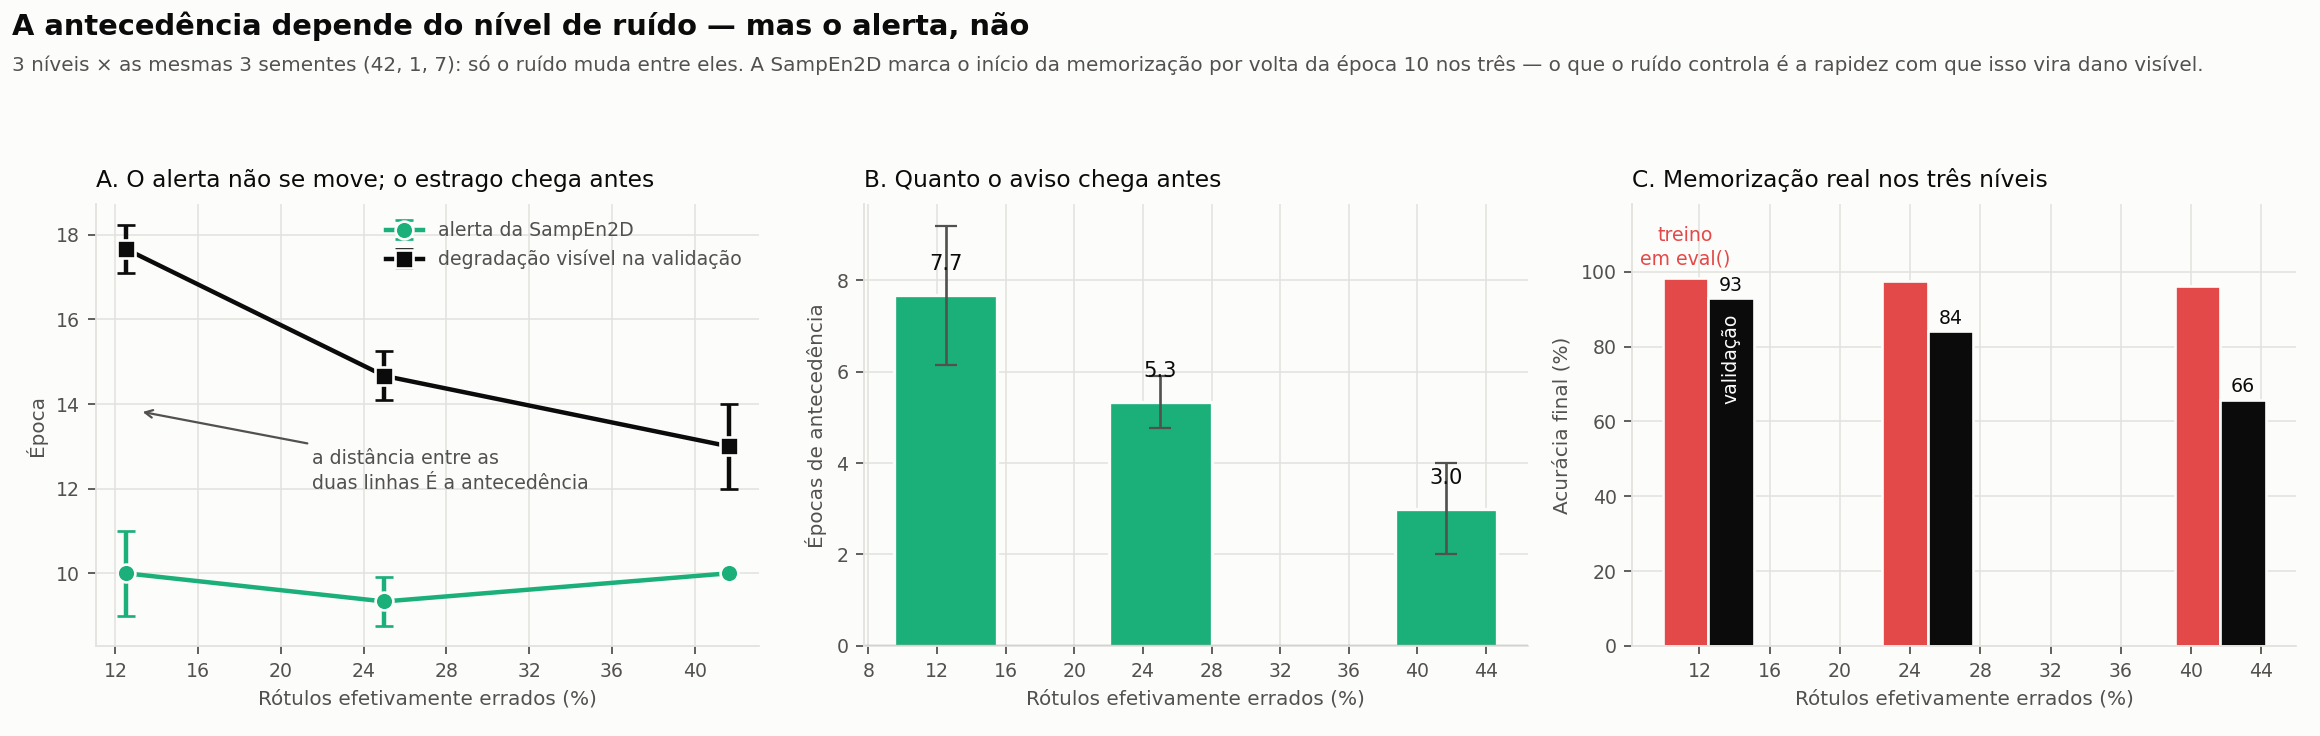
\includegraphics[width=0.9\textwidth]{figures/d2_niveis_ruido.png}
    \caption{Época do alerta e época da âncora em função do nível de corrupção
    de rótulos. A época do alerta é estável; a da âncora antecipa-se com o
    aumento da corrupção.}
    \label{fig:d2-niveis}
    \fonte{Elaborado pelo autor.}
\end{figure}

\subsection{Generalização para outra arquitetura}
\label{sec:res-d2-arquitetura}

O experimento foi repetido com a DenseNet-121, com oito execuções com
corrupção e cinco controles pareados. Os resultados constam da
Tabela~\ref{tab:d2-densenet}.

\begin{table}[H]
\centering
\caption{Resultados na DenseNet-121, com oito execuções com corrupção e cinco
controles pareados.}
\label{tab:d2-densenet}
\small
\begin{tabular}{lccc}
\toprule
\textbf{Indicador} & \textbf{Razão de amplitude} & \textbf{$p$} &
\textbf{Antecedência (épocas)} \\
\midrule
LMC       & $1{,}06$ & $0{,}435$   & --- \\
SampEn 1D & $1{,}77$ & $0{,}00155$ & $22{,}50 \pm 2{,}33$ \\
SampEn2D  & $4{,}35$ & $0{,}00155$ & $21{,}12 \pm 2{,}36$ \\
\bottomrule
\end{tabular}
\fonte{Elaborado pelo autor.}
\end{table}

O achado central replica-se na segunda arquitetura. A SampEn2D discrimina com
razão de $4{,}35$ vezes ($p = \num{0,00155}$) e a antecedência é
consideravelmente maior, de $21{,}1 \pm 2{,}4$ épocas, com intervalo de
confiança de \SI{95}{\percent} entre $19{,}2$ e $23{,}1$. A LMC, de novo, não
discrimina ($p = \num{0,435}$), o que reforça a consistência desse resultado
negativo entre arquiteturas.

Duas ressalvas, porém, devem ser explicitadas.

A primeira é que a razão de amplitude é menor do que na ResNet-18
($4{,}35$ contra $5{,}65$), e a SampEn 1D, que discriminava na ResNet, passa a
ter poder marginal ($1{,}77$). O contraste, portanto, replica-se em direção,
mas não em magnitude.

A segunda é mais relevante e não deve ser omitida: \textbf{na DenseNet-121 a
época do sinal não separa os grupos}. As execuções com corrupção inflectem nas
épocas $\{8,9,9,9,9,11,11,12\}$, enquanto os controles pareados inflectem em
$\{7,8,10,16,25\}$ --- três deles, portanto, tão cedo ou mais cedo que as
execuções com corrupção. Na ResNet-18 a separação temporal é quase perfeita; na
DenseNet-121, não existe. O que discrimina nessa arquitetura é a
\emph{amplitude} da variação, não o \emph{momento} em que ela começa. A
consequência prática é direta: um monitor que emita alerta pelo simples cruzamento
de um limiar temporal produziria falsos positivos na DenseNet-121, e o critério
precisa incorporar a magnitude.

\begin{figure}[H]
    \centering
    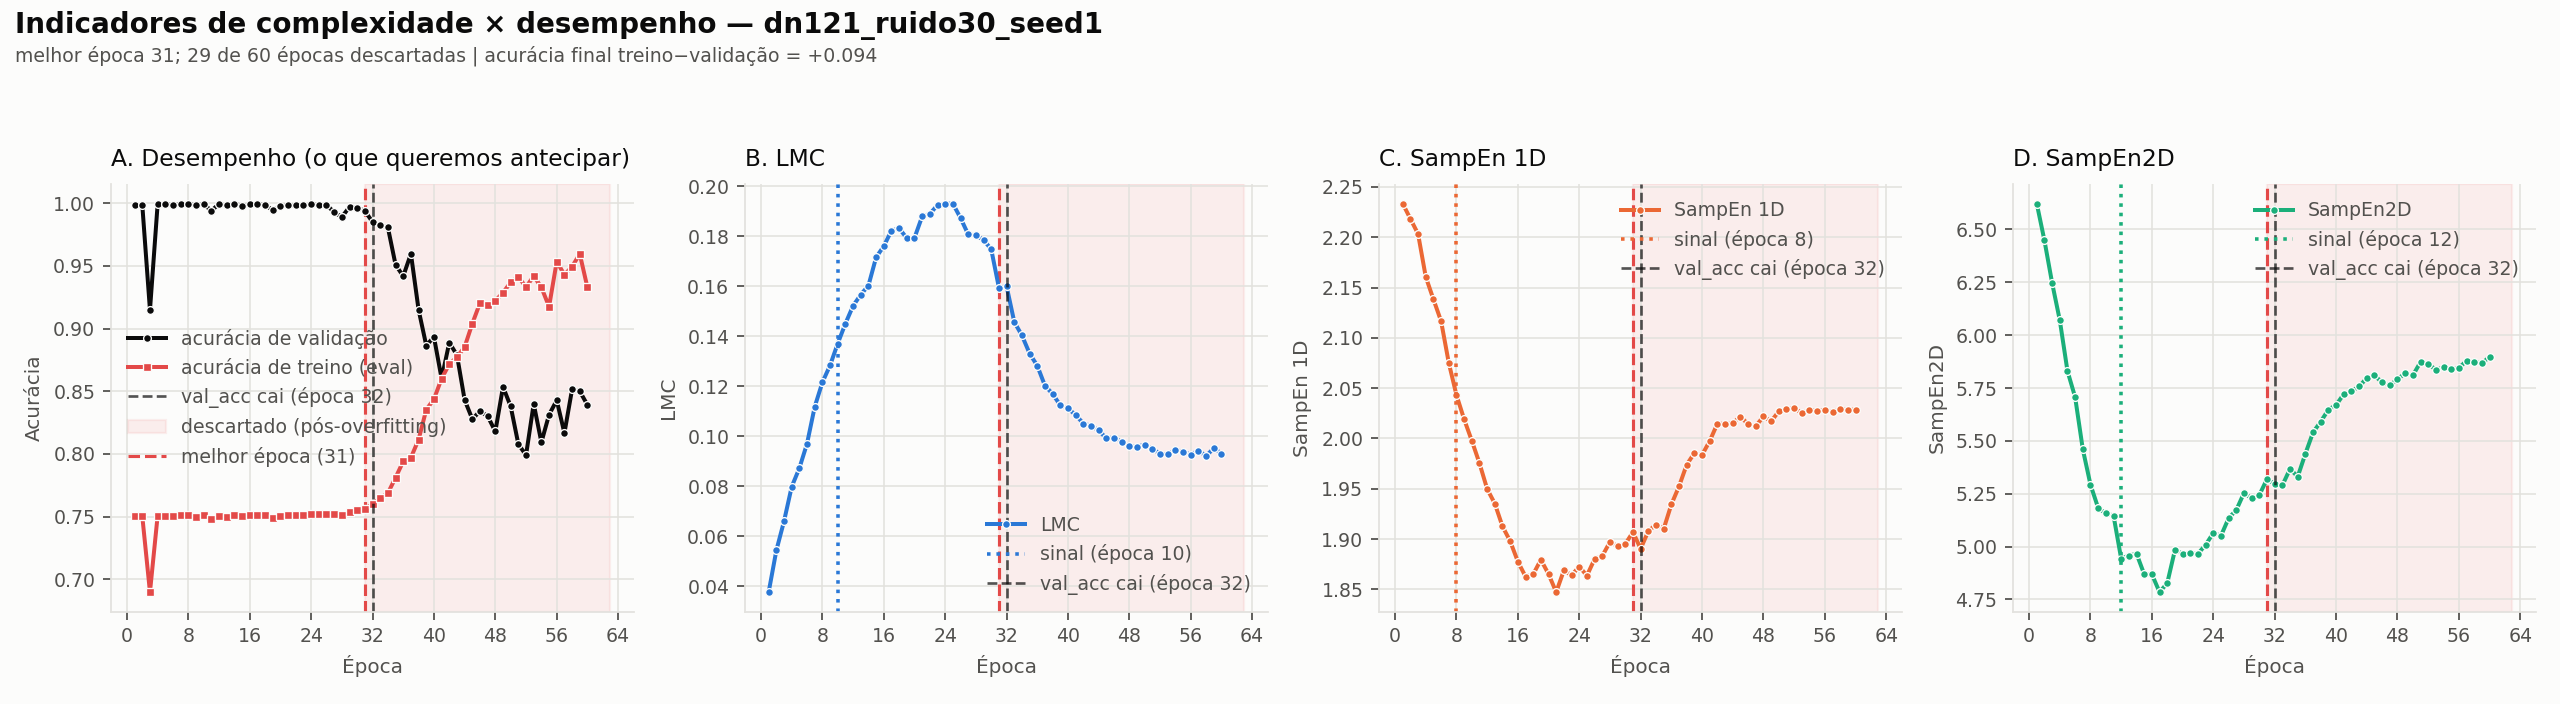
\includegraphics[width=0.95\textwidth]{figures/d2_indicadores_dn121.png}
    \caption{Trajetória dos indicadores na camada densa da DenseNet-121, em
    execução com corrupção de rótulos.}
    \label{fig:d2-dn121}
    \fonte{Elaborado pelo autor.}
\end{figure}

\subsection{Ablação da ordem de achatamento}
\label{sec:res-d2-ablacao}

A Seção~\ref{sec:camada-densa} fixou a ordem por neurônio como convenção
padrão, por coerência com a decisão D2, e previu o reporte da comparação com a
ordem por entrada. A Tabela~\ref{tab:d2-ablacao} apresenta o resultado, obtido
sobre cinco execuções com corrupção e cinco controles.

\begin{table}[H]
\centering
\caption{Comparação das duas ordens de achatamento na SampEn 1D da camada densa.}
\label{tab:d2-ablacao}
\small
\begin{tabular}{lcc}
\toprule
\textbf{Ordem} & \textbf{Razão de amplitude} & \textbf{Antecedência (épocas)} \\
\midrule
Por neurônio (padrão adotado) & $3{,}52$ & $3{,}6$ \\
Por entrada                   & $7{,}73$ & $7{,}4$ \\
\bottomrule
\end{tabular}
\fonte{Elaborado pelo autor.}
\end{table}

O resultado contraria a convenção adotada, e isso precisa ser dito sem
atenuação: a leitura \emph{por entrada} é superior nos dois critérios,
discriminando mais que o dobro ($7{,}73$ contra $3{,}52$) e avisando com o dobro
da antecedência ($7{,}4$ contra $3{,}6$ épocas).

Há uma explicação plausível. Percorrer a matriz por entrada agrupa, para cada
característica, os pesos que ela envia a \emph{todas} as classes --- e é
exatamente aí que a memorização se manifesta, quando uma característica passa a
apontar de forma desproporcional para uma classe específica. Percorrendo por
neurônio, esse contraste dilui-se ao longo das \num{512} posições do campo
receptivo.

Registre-se que o efeito prático dessa escolha é limitado, pois o indicador de
melhor desempenho neste trabalho é a SampEn2D, que não achata a matriz e
preserva as duas direções simultaneamente. A discussão de ordem afeta apenas a
variante unidimensional. Ainda assim, a evidência recomenda reconsiderar a
convenção adotada.

\subsection{Sobre o pareamento dos controles}
\label{sec:res-d2-pareamento}

Um aspecto metodológico merece registro explícito, por afetar a validade de
todos os números desta seção.

Em uma versão anterior deste conjunto de experimentos, as execuções de controle
não eram estritamente pareadas: além de não terem rótulos corrompidos, elas
empregavam aumento de dados, decaimento de pesos de $10^{-4}$ e horizonte de
\num{40} épocas, contra ausência de aumento, decaimento nulo e \num{60} épocas
nas execuções com corrupção. Como aumento de dados e decaimento de pesos são,
ambos, formas de regularização que reduzem sobreajuste por conta própria, o
contraste medido era atribuível a mais de uma causa, e não exclusivamente à
memorização.

Todo o conjunto de controles foi então refeito com pareamento estrito, e os
números reportados nesta seção são os dessa segunda versão. A comparação entre
as duas consta da Tabela~\ref{tab:d2-pareamento}.

\begin{table}[H]
\centering
\caption{Efeito da correção do pareamento sobre as razões de amplitude da
SampEn2D.}
\label{tab:d2-pareamento}
\small
\begin{tabular}{lccc}
\toprule
\textbf{Arquitetura} & \textbf{Controles não pareados} &
\textbf{Controles pareados} & \textbf{$p$ final} \\
\midrule
ResNet-18    & $5{,}71$ ($n=8$) & $5{,}65$ ($n=8$) & $0{,}00016$ \\
DenseNet-121 & $2{,}80$ ($n=3$) & $4{,}35$ ($n=8$) & $0{,}00155$ \\
\bottomrule
\end{tabular}
\fonte{Elaborado pelo autor.}
\end{table}

Na ResNet-18 a razão praticamente não se alterou, passando de $5{,}71$ para
$5{,}65$. Esse é um resultado importante em si: como a correção removeu a
regularização dos controles e o contraste permaneceu, conclui-se que o efeito
medido decorre da memorização, e não das diferenças de regularização. Na
DenseNet-121 a razão \emph{aumentou}, de $2{,}80$ para $4{,}35$, e passou a ser
estatisticamente significativa --- o que indica que a aparente fraqueza dessa
arquitetura, registrada em análise preliminar, era em boa parte artefato do
pareamento inadequado, agravado pelo número reduzido de execuções.

%% capitulos/conclusao.tex

\chapter{Conclusão}
\label{ch:conclusao}

Este trabalho descreveu como a complexidade estatística dos pesos da camada
densa de redes neurais profundas se comporta durante o treinamento, no contexto
de classificação de imagens médicas com a arquitetura ResNet-18 e o conjunto
MedNIST. A abordagem articulou duas medidas complementares --- a complexidade
LMC \cite{lmc1995} e a entropia amostral SampEn \cite{richman2000} ---
calculadas a cada época sobre a camada densa, em execuções de controle, com
subamostragem do conjunto de treino e com ruído branco e rosa nas imagens de
treino.

\section{Principais achados}
\label{sec:conc-achados}

\pendente{síntese do comportamento da LMC e da SampEn em cada regime, a partir
do Capítulo~\ref{ch:resultados}.}

\section{Trabalhos Futuros}
\label{sec:futuros}

A partir das limitações identificadas, perfilam-se os desdobramentos abaixo.

\begin{enumerate}
  \item \textbf{Repositório de maior dificuldade.} Repetir os experimentos em
  um conjunto de dados menos saturável que o MedNIST, no qual a perda de
  generalização seja mais pronunciada, e comparar sobre a camada densa os mesmos
  regimes de treinamento.

  \item \textbf{Ordem de achatamento.} A SampEn$_{1D}$ depende da ordem em que
  a matriz da camada densa é achatada (Seção~\ref{sec:camada-densa}). Convém
  comparar a ordem por neurônio, adotada como padrão, com a ordem por entrada.

  \item \textbf{Análise multiescala} (MSE) \cite{costa2002,costa2005}
  dos pesos da camada densa, para investigar dependências em diferentes
  escalas.

  \item \textbf{Comparação com outras arquiteturas} (EfficientNet,
  Wide ResNet) para verificar se o comportamento observado na ResNet-18
  se mantém.

  \item \textbf{Análise de sensibilidade à regularização explícita}
  (\emph{weight decay}, \emph{dropout}, \emph{label smoothing}) para
  testar se a manipulação dirigida da propensão ao sobreajuste altera o
  comportamento das medidas na camada densa.

  \item \textbf{Dados substitutos (\emph{surrogate data})} como teste de
  hipótese nula sobre a trajetória de complexidade, permitindo
  caracterizar o quanto da estrutura observada se afasta do
  comportamento esperado sob inicialização aleatória mais ruído.

  \item \textbf{Uso prático.} Avaliar, a partir do comportamento descrito,
  se as medidas podem compor um critério auxiliar de parada em pipelines de
  treinamento, comparando custo computacional e desempenho com os critérios
  tradicionais baseados na perda de validação.
\end{enumerate}


%% ─── Referências ─────────────────────────────────────────────────────────────
\postextual
\bibliography{referencias}

%% ─── Apêndices ───────────────────────────────────────────────────────────────
\begin{apendicesenv}
\partapendices
%% apendices/exemplo_numerico.tex
%% Apêndice A — Exemplo numérico da ordem de achatamento da camada densa

\chapter{Exemplo numérico da ordem de achatamento da camada densa}
\label{ap:exemplo-numerico}

Este apêndice complementa a Seção~\ref{sec:camada-densa}, rastreando,
elemento a elemento, a correspondência entre a matriz de pesos de uma camada
\texttt{Linear} do PyTorch e a sequência linear sobre a qual a SampEn$_{1D}$ é
calculada. Usa-se uma camada mínima, $2 \times 3$, primeiro na ordem por
neurônio (Equação~\ref{eq:ordem-neuronio}) e em seguida na ordem por entrada
(Equação~\ref{eq:ordem-entrada}).

% ===========================================================================
\section{Camada Linear: matriz \texorpdfstring{$2 \times 3$}{2x3}}
\label{sec:ap-linear}

Considere uma camada \texttt{nn.Linear(in\_features=3, out\_features=2)}
cujo tensor \texttt{weight} de \emph{shape} $[\mathrm{Out}, \mathrm{In}] = [2, 3]$
recebe valores inteiros para facilitar o rastreamento:
\begin{equation}
  W_{\text{lin}} \;=\;
  \begin{pmatrix}
    w_{0,0} & w_{0,1} & w_{0,2} \\
    w_{1,0} & w_{1,1} & w_{1,2}
  \end{pmatrix}
  \;=\;
  \begin{pmatrix}
    1 & 2 & 3 \\
    4 & 5 & 6
  \end{pmatrix}.
\end{equation}

Aplicando \texttt{W\_lin.flatten()} obtemos o vetor

\begin{equation}
  W_{\text{lin}}.\texttt{flatten()} \;=\; [\,1,\;2,\;3,\;4,\;5,\;6\,].
\end{equation}

A Tabela~\ref{tab:ap-linear} mostra a correspondência elemento a elemento.
Note que a leitura é feita \textbf{linha por linha}: primeiro saem todos os
três pesos de entrada do neurônio de saída $\mathrm{Out}=0$, depois os três
pesos do neurônio $\mathrm{Out}=1$. Cada linha contígua do vetor
corresponde a \emph{um único neurônio de saída}.

\begin{table}[H]
\centering
\caption{Mapeamento elemento a elemento da camada Linear $2 \times 3$.}
\label{tab:ap-linear}
\small
\begin{tabular}{cccccc}
\toprule
\textbf{Posição no vetor} & 0 & 1 & 2 & 3 & 4 \\
                          & ($\to$) 5 & & & & \\
\midrule
\textbf{Elemento}      & $w_{0,0}$ & $w_{0,1}$ & $w_{0,2}$ & $w_{1,0}$ & $w_{1,1}$ \\
                       & $w_{1,2}$ & & & & \\
\midrule
\textbf{Valor}         & 1 & 2 & 3 & 4 & 5 \\
                       & 6 & & & & \\
\midrule
\textbf{Pertence a}    & \multicolumn{3}{c}{\textbf{Saída $\mathrm{Out}=0$}} & \multicolumn{2}{c}{\textbf{Saída $\mathrm{Out}=1$}} \\
\bottomrule
\end{tabular}
\end{table}

% ===========================================================================
\section{Contraste: ordem por entrada}
\label{sec:ap-transposicao}

Transpondo a mesma matriz antes do achatamento, percorrem-se primeiro todos os
pesos que partem da entrada $\mathrm{In}=0$, depois os da entrada
$\mathrm{In}=1$, e assim por diante:

\begin{equation}
  W_{\text{lin}}^{\top}.\texttt{flatten()} \;=\; [\,1,\;4,\;2,\;5,\;3,\;6\,].
\end{equation}

Os dois vetores contêm exatamente os mesmos seis valores, e portanto o mesmo
histograma: a complexidade LMC é idêntica nas duas ordens. O que muda é a
vizinhança de cada valor, à qual a SampEn$_{1D}$ é sensível.

% ===========================================================================
\section{Reprodutibilidade}
\label{sec:ap-reproducao}

Os vetores apresentados neste apêndice podem ser reproduzidos diretamente em
PyTorch:

\begin{verbatim}
    import torch

    # Linear (Out=2, In=3)
    W_lin = torch.tensor([[1., 2., 3.],
                          [4., 5., 6.]])
    print(W_lin.flatten().tolist())      # ordem por neuronio
    # [1.0, 2.0, 3.0, 4.0, 5.0, 6.0]
    print(W_lin.t().flatten().tolist())  # ordem por entrada
    # [1.0, 4.0, 2.0, 5.0, 3.0, 6.0]
\end{verbatim}

%% apendices/validacao_numerica.tex
%% Apêndice B — Validação numérica das medidas de complexidade

\chapter{Validação numérica das medidas de complexidade}
\label{ap:validacao-numerica}

Este apêndice cumpre a parte do objetivo específico~1
(\autoref{ch:introducao}) referente à \emph{validação numérica das medidas
em casos analiticamente conhecidos}. As implementações descritas na
\autoref{sec:medidas} --- complexidade LMC e \emph{Sample Entropy} 1D e 2D ---
são aplicadas a distribuições e séries cujo comportamento esperado é conhecido
em forma fechada ou qualitativamente, verificando-se que os valores produzidos
coincidem com a teoria. Todos os resultados desta seção são reproduzíveis
executando \texttt{scripts/validacao\_numerica.py} (semente $42$,
\texttt{numpy}~1.26); para a LMC fixou-se $N = 100$ \emph{bins}, de modo que a
entropia da uniforme tem valor de referência $\log_2 N \approx 6{,}6439$~bits.

% ===========================================================================
\section{Complexidade LMC}
\label{sec:ap-validacao-lmc}

Para a forma adotada $C = H \times D$, com $H$ em bits e
$D = \sum_i (p_i - 1/N)^2$, os dois extremos têm valor analítico exato: a
distribuição \emph{uniforme} maximiza a entropia ($H = \log_2 N$) e anula o
desequilíbrio ($D = 0$), enquanto a distribuição \emph{degenerada} (toda a massa
em um único \emph{bin}) anula a entropia ($H = 0$) e atinge
$D = 1 - 1/N$; em ambos os casos $C = 0$. Uma distribuição \emph{gaussiana}
representa o regime intermediário, com $0 < H < \log_2 N$, $D > 0$ e,
portanto, $C > 0$. A \autoref{tab:val-lmc} confirma os três comportamentos.

\begin{table}[H]
  \centering
  \caption{Validação da LMC ($N = 100$ \emph{bins}). Os casos uniforme e
  degenerado reproduzem os valores analíticos com precisão de máquina.}
  \label{tab:val-lmc}
  \begin{tabular}{lrrrl}
    \toprule
    Distribuição & $H$ (bits) & $D$ & $C = H\times D$ & Esperado \\
    \midrule
    Uniforme            & $6{,}6439$ & $0{,}00000$ & $0{,}00000$ & $H=\log_2 N,\ D\approx0,\ C\approx0$ \\
    Degenerada          & $0{,}0000$ & $0{,}99000$ & $0{,}00000$ & $H=0,\ D=1-1/N,\ C=0$ \\
    Gaussiana           & $5{,}4638$ & $0{,}01646$ & $0{,}08994$ & $0<H<\log_2 N,\ D>0,\ C>0$ \\
    \bottomrule
  \end{tabular}
\end{table}

% ===========================================================================
\section{Sample Entropy 1D}
\label{sec:ap-validacao-sampen1d}

Com $m = 2$ e $r = 0{,}2\,\sigma$, uma série \emph{constante} é
perfeitamente regular e produz $\mathrm{SampEn} = 0$ por definição; uma série
\emph{periódica} é altamente previsível e produz valor próximo de zero;
\emph{ruído branco gaussiano} maximiza a irregularidade e produz um valor finito
e elevado, da ordem de $2{,}1$ --- compatível com o reportado na literatura para
sinais sem estrutura sob essa parametrização. A \autoref{tab:val-sampen1d}
confirma a ordenação esperada.

\begin{table}[H]
  \centering
  \caption{Validação da SampEn 1D ($m = 2$, $r = 0{,}2\,\sigma$, séries de
  $1000$ amostras).}
  \label{tab:val-sampen1d}
  \begin{tabular}{lrl}
    \toprule
    Série & SampEn & Esperado \\
    \midrule
    Constante                 & $0{,}0000$ & $0$ (perfeitamente regular) \\
    Periódica (seno, $T=20$)  & $0{,}1864$ & $\approx 0$ (previsível) \\
    Ruído branco gaussiano    & $2{,}0934$ & finito e elevado (irregular) \\
    \bottomrule
  \end{tabular}
\end{table}

% ===========================================================================
\section{Sample Entropy 2D}
\label{sec:ap-validacao-sampen2d}

A SampEn 2D preserva os limites esperados: uma matriz \emph{constante}
produz $0$, e uma matriz com \emph{estrutura periódica} produz valor baixo.
Para \emph{ruído branco} $64 \times 64$, a tolerância padrão $r = 0{,}2\,\sigma$
satura em $+\infty$ --- nenhum par de janelas $(m+1)\times(m+1)$ casa dentro da
tolerância ---, exatamente o comportamento que motivou a adoção de
$r = 0{,}5\,\sigma$ na \autoref{sec:medidas-extensoes}; sob essa tolerância o
valor torna-se finito ($\approx 6{,}46$). A validação, portanto, não apenas
confirma os limites como reproduz de forma independente a justificativa
metodológica para a calibração de $r$ no caso 2D.

\begin{table}[H]
  \centering
  \caption{Validação da SampEn 2D ($m = 2$, matrizes $64 \times 64$). O caso
  do ruído sob $r = 0{,}2\,\sigma$ reproduz a saturação que motiva
  $r = 0{,}5\,\sigma$.}
  \label{tab:val-sampen2d}
  \begin{tabular}{lrl}
    \toprule
    Matriz & SampEn 2D & Esperado \\
    \midrule
    Constante                    & $0{,}0000$ & $0$ (regular) \\
    Estrutura periódica          & $0{,}8173$ & baixa (estruturada) \\
    Ruído branco ($r=0{,}2\,\sigma$) & $+\infty$ & satura (motiva $r=0{,}5\,\sigma$) \\
    Ruído branco ($r=0{,}5\,\sigma$) & $6{,}4636$ & finito e elevado (irregular) \\
    \bottomrule
  \end{tabular}
\end{table}

Em conjunto, as três validações estabelecem que as implementações reproduzem os
valores analíticos exatos nos extremos (LMC nas distribuições uniforme e
degenerada; SampEn em séries constantes) e a ordenação qualitativa esperada nos
regimes intermediários, sustentando o uso das medidas nas análises do
\autoref{ch:resultados}.

\end{apendicesenv}

\end{document}
